%%%%%%%%%%%%%%%%%%%%%%%%%%%%%%%%%%%%%%%%%%%%%%%%%%%%%%%%%
%%             东南大学数电实验报告 LaTeX 模板
%%               Experiment 3 Report.tex
%% https://github.com/Teddy-van-Jerry/SEU_Digital_Report
%% ======================================================
%% 版本信息:
%% v1.0 (Nov. 07, 2021)
%% ------------------------------------------------------
%% 模板制作:
%% Teddy van Jerry, (me@teddy-van-jerry.org)
%% * GitHub: https://github.com/Teddy-van-Jerry
%% * Website: https://teddy-van-jerry.org
%% * Blog: https://blog.teddy-van-jerry.org
%% ------------------------------------------------------
%% 使用说明:
%% 1. 编译使用 XeLaTeX 和 Biber
%% 2. 报告基本信息通过修改导言区以 exp 开头的命令
%% 3. 参考文献位于 ref/ref.bib
%% 4. 报告模板依据 MIT License 开源共享
%% ------------------------------------------------------
%% Copyright 2021 (c) Teddy van Jerry
%%
%% Permission is hereby granted, free of charge, to any
%% person obtaining a copy of this software and
%% associated documentation files (the "Software"), to
%% deal in the Software without restriction, including
%% without limitation the rights to use, copy, modify,
%% merge, publish, distribute, sublicense, and/or sell
%% copies of the Software, and to permit persons to whom
%% the Software is furnished to do so, subject to the
%% following conditions:
%%
%% The above copyright notice and this permission notice
%% shall be included in all copies or substantial
%% portions of the Software.
%% 
%% THE SOFTWARE IS PROVIDED "AS IS", WITHOUT WARRANTY OF
%% ANY KIND, EXPRESS OR IMPLIED, INCLUDING BUT NOT
%% LIMITED TO THE WARRANTIES OF MERCHANTABILITY, FITNESS
%% FOR A PARTICULAR PURPOSE AND NONINFRINGEMENT. IN NO
%% EVENT SHALL THE AUTHORS OR COPYRIGHT HOLDERS BE LIABLE
%% FOR ANY CLAIM, DAMAGES OR OTHER LIABILITY, WHETHER IN
%% AN ACTION OF CONTRACT, TORT OR OTHERWISE, ARISING
%% FROM, OUT OF OR IN CONNECTION WITH THE SOFTWARE OR THE
%% USE OR OTHER DEALINGS IN THE SOFTWARE.
%%%%%%%%%%%%%%%%%%%%%%%%%%%%%%%%%%%%%%%%%%%%%%%%%%%%%%%%%%

%% 使用实验报告模板类(字体大小 11pt 约为五号字)
\documentclass[11pt]{SEU-Digital-Report}

%%%%%%%%%%%%%%%%%%%% 报告基本信息 %%%%%%%%%%%%%%%%%%%%
\expno{四} % 实验序号
\expname{数字模块设计与验证} % 实验名称
\expauthor{赵舞穹} % 姓名
\expID{61520522} % 学号
\expmates{郑瑞琪} % 同组
\expmatesID{61520523} % 学号(同组)
\expmajor{工科试验班} % 专业
\explab{计算机硬件技术} % 实验室
\expdate{2021年11月19日} % 实验日期
\expreportdate{2021年11月29日} % 实验日期
\expgrade{} % 成绩评定
\exptutor{冯熳} % 评阅教师
%%%%%%%%%%%%%%%%%%%%%%%%%%%%%%%%%%%%%%%%%%%%%%%%%%%%

\usepackage{pgfplots}
\pgfplotsset{compat=1.11}

%% 报告正文
\begin{document}
  % 打印封面页
  \exptitlepage

  \tableofcontents
  \newpage

  \section{实验目的}
        
    \begin{enumerate}
        \item 通过实验学习理解和掌握虚拟器件/接口、IP 和基于平台的数字系统设计方法,形
        成软核和硬核、宏单元、虚拟器件、IP 设计及验证的概念和基本的调用构建过程;
        \item 通过实践加深对可编程数字系统模块概念的正确理解,进一步熟悉掌握FPGA 数字
        模块的仿真验证方法和开发设计过程及FPGA 硬件演示应用方法,初步理解掌握Xilinx 的
        IP 核和Altera 的参数化宏功能模块库(Library of Parameterized Modules--LPM)的原理,
        分析对比计算机典型数字元件模块功能设计和典型应用方法,总结形成计算机系统与接口
        相关模块可能的HDL 实现方法。
    \end{enumerate}

  \section{实验内容}

    \subsection{XILINX Vivado 加减法器的实现}

      \subsubsection{Verilog 模块调用IP 核搭建}

        首先如图~\ref{fig:IP_add_sub_8} 配置好一个 \texttt{Adder/Subtracter} 的 IP 核,这样就相当于完成了整个模块而没有具体的写出代码.

        \begin{figure}[htbp]
          \centering
          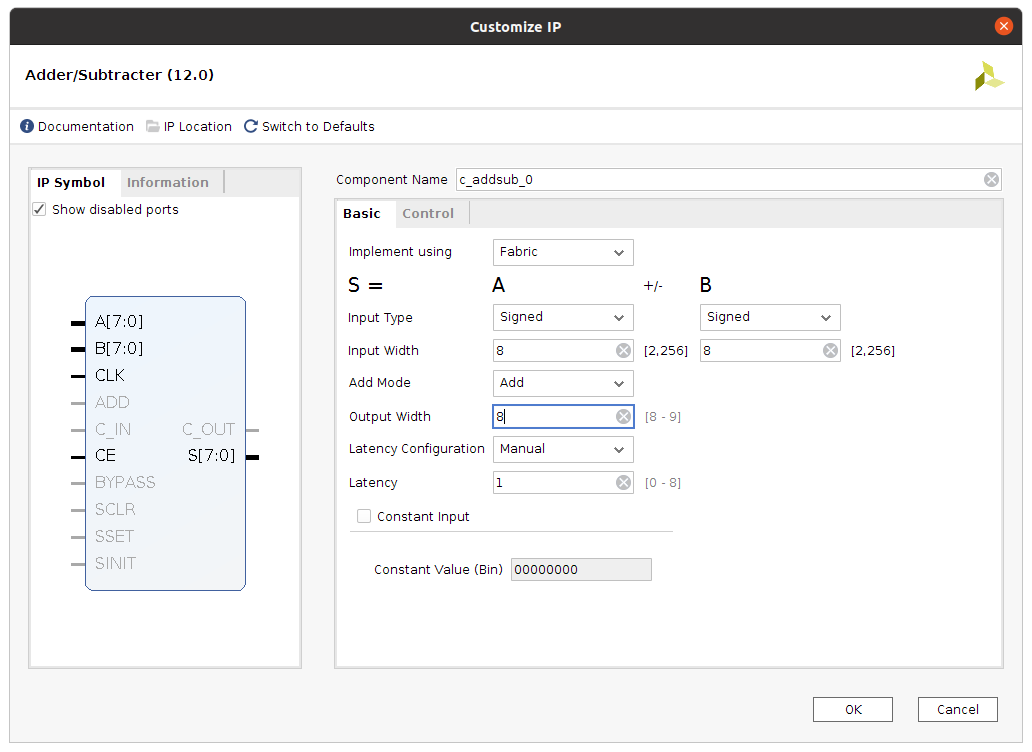
\includegraphics[width=.6\linewidth]{fig/IP_add_sub_8.png}
          \caption{Vivado 中设置8位\texttt{Adder/Subtracter} 模块}
          \label{fig:IP_add_sub_8}
        \end{figure}

        随后需要添加 testbench 代码,此处借鉴老师提供的 \texttt{demo.v}\cite{guide}.

        \begin{lstlisting}[language=verilog]
module tvj_demo( // use my symbol 'tvj'
  input t1, 
  output t2 
  ); 
  reg [7:0] Am,Bm; 
  wire [7:0] Sm; 
  reg CLKm=0,CEm=0; 
  c_addsub_1 myadder ( 
  .A(Am),     // input wire [7 : 0] A
  .B(Bm),     // input wire [7 : 0] B
  .CLK(CLKm), // input wire CLK
  .CE(CEm),   // input wire CE
  .S(Sm)      // output wire [7 : 0] S
  );
  always #2 CLKm = ~CLKm; // clock signal
  initial begin
    #2;
    CEm = 1;
    Am = 38;
    Bm = 88;
    #6; 
    Am = 55;
    Bm = -24;
    #5;
    Am = -70;
    Bm = -38;
    #5;
    CEm = 0;
    Am = 8'b1011001;
    Bm = 8'b11010001;
    #20;
  end
endmodule
        \end{lstlisting}

        进行 Behavioral Simulation,得到的行为仿真图如图~\ref{fig:IP_simu} 所示.
        \begin{analyze}{行为仿真结果}{}
          行为仿真结果显示它成功进行了 8 位有符号数(即按照补码编码)的和差运算.
        \end{analyze}

        \begin{figure}[htbp]
          \centering
          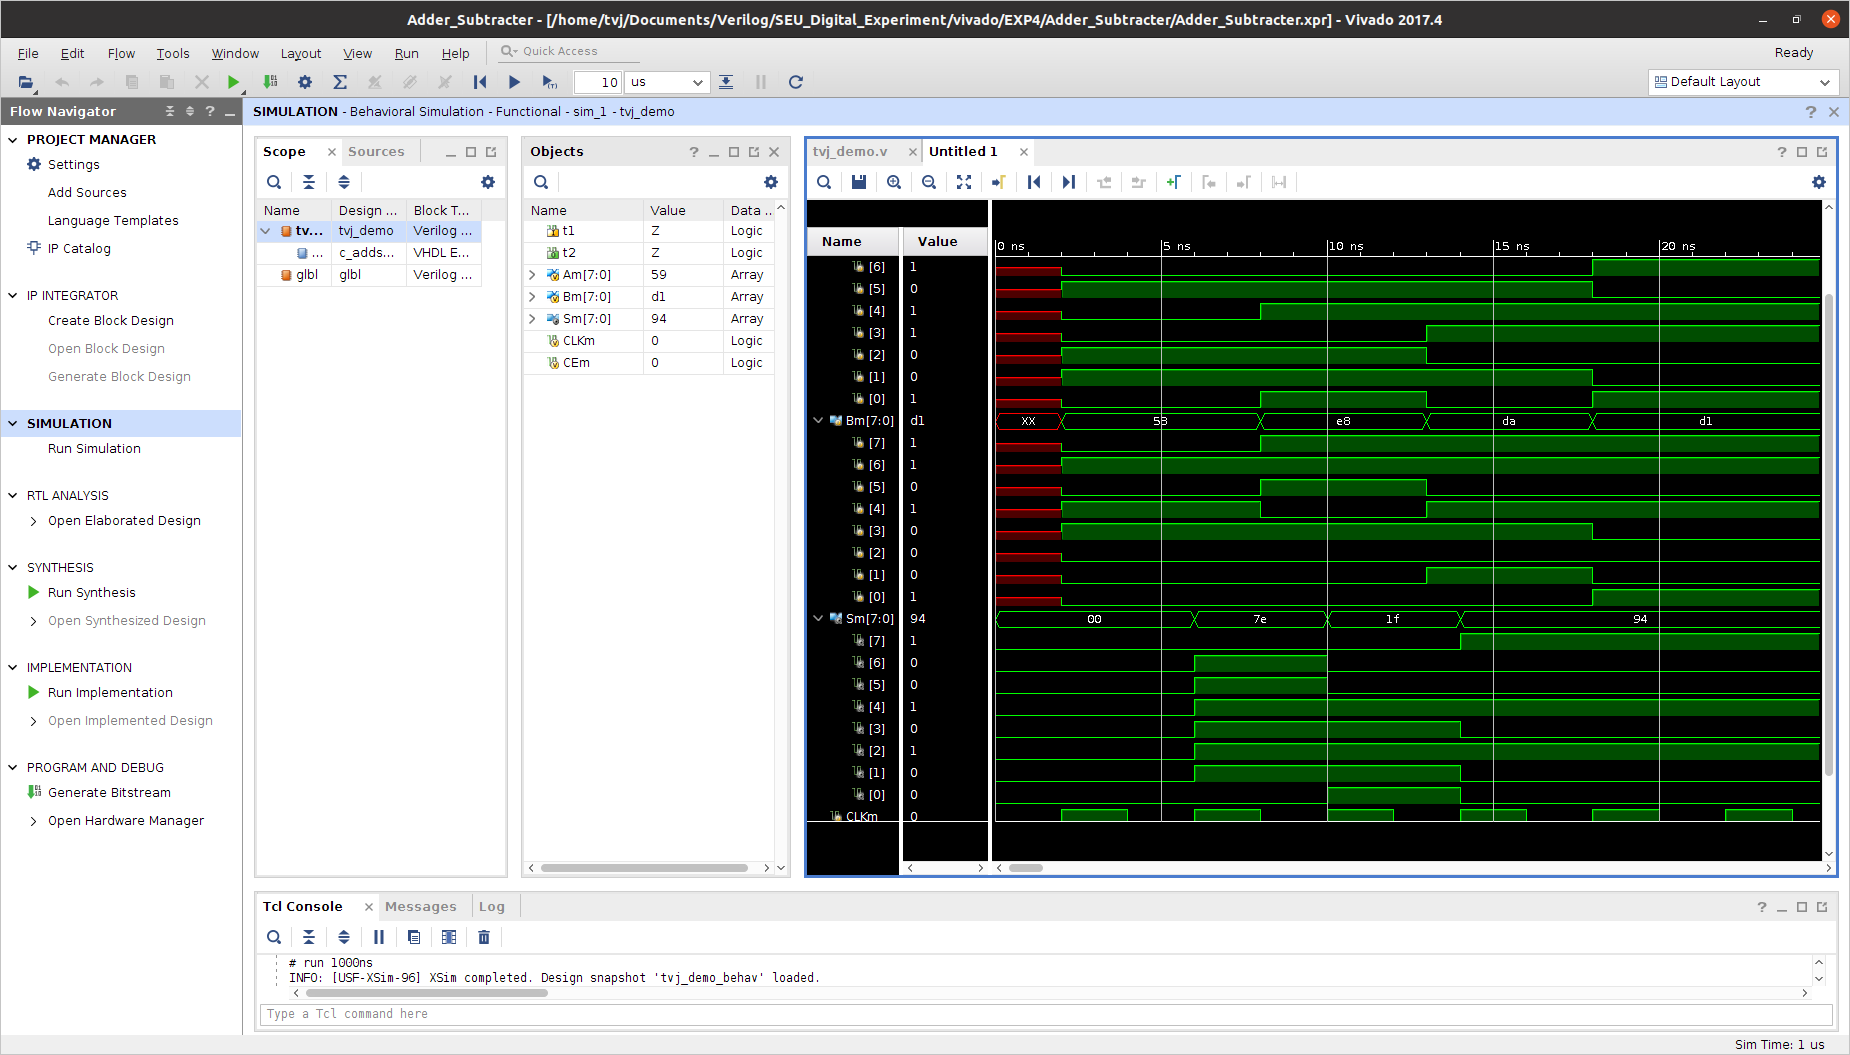
\includegraphics[width=\linewidth]{fig/IP_simu.png}
          \caption{行为仿真图}
          \label{fig:IP_simu}
        \end{figure}

        分别完成 RTL,Synthesis,Implementation 的仿真,分别得到图~\ref{fig:IP_RTL},\ref{fig:IP_sys},\ref{fig:IP_imp} 的结果.
        \begin{analyze}{RTL,Synthesis,Implementation 的仿真}{}
          RTL级仿真是寄存器级的,而我们将其展开,如图~\ref{fig:IP_RTL_detailed} 所示,是嵌套的具有超前进位的结构并不需要使用到寄存器.
          Synthesis(综合)则需要将更多的内容考虑到了,例如具体的输入输出始时钟上存在一定的差异.
          Implementation(实现)需要考虑到具体开发板的情况,我在创建项目的时候是按照默认选择的. Implementation 会完成 Translation,Mapping,Place\&Route 的工作,这些是在 Synthesis 中没有的.
          图~\ref{fig:IP_imp} 结构如此简单我认为可能是对应的板子本身就具有 \texttt{Adder/Subtracter}.
        \end{analyze}        

        \begin{figure}[htbp]
          \centering
          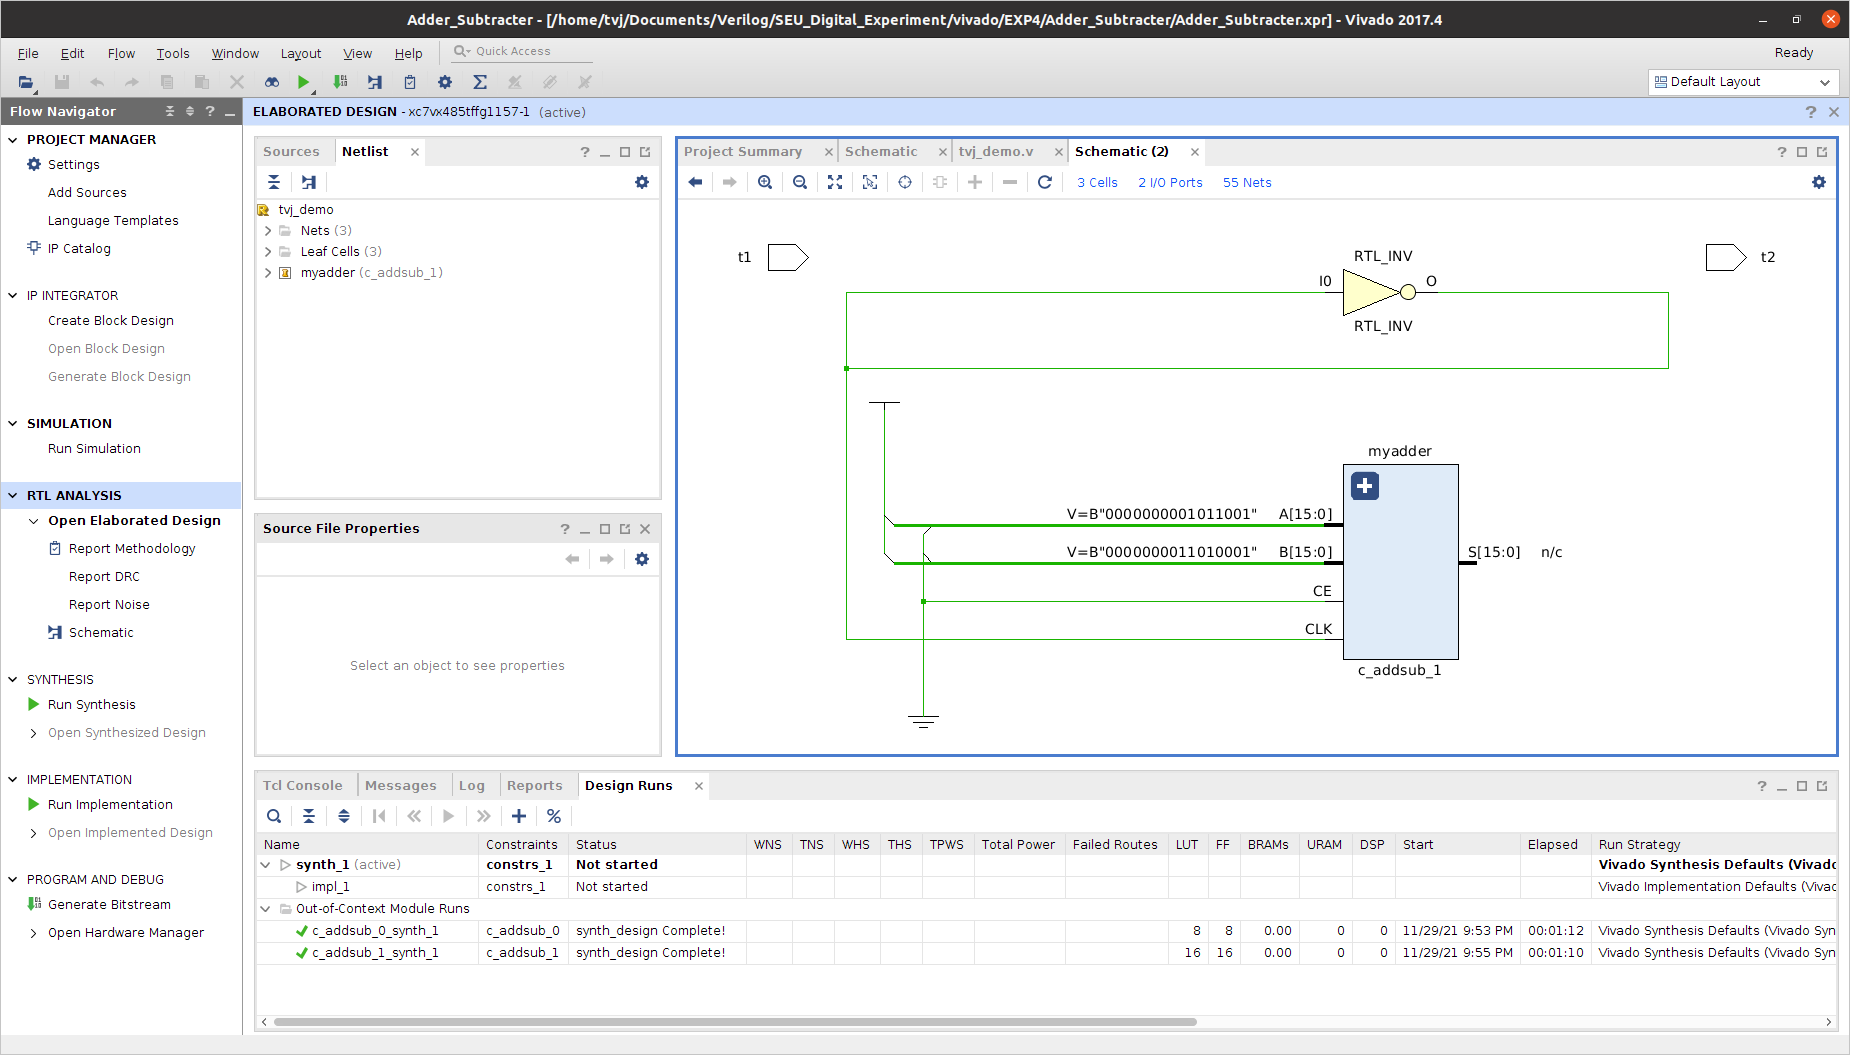
\includegraphics[width=\linewidth]{fig/IP_RTL.png}
          \caption{RTL 级电路}
          \label{fig:IP_RTL}
        \end{figure}

        \newpage
        \begin{figure}[htbp]
          \centering
          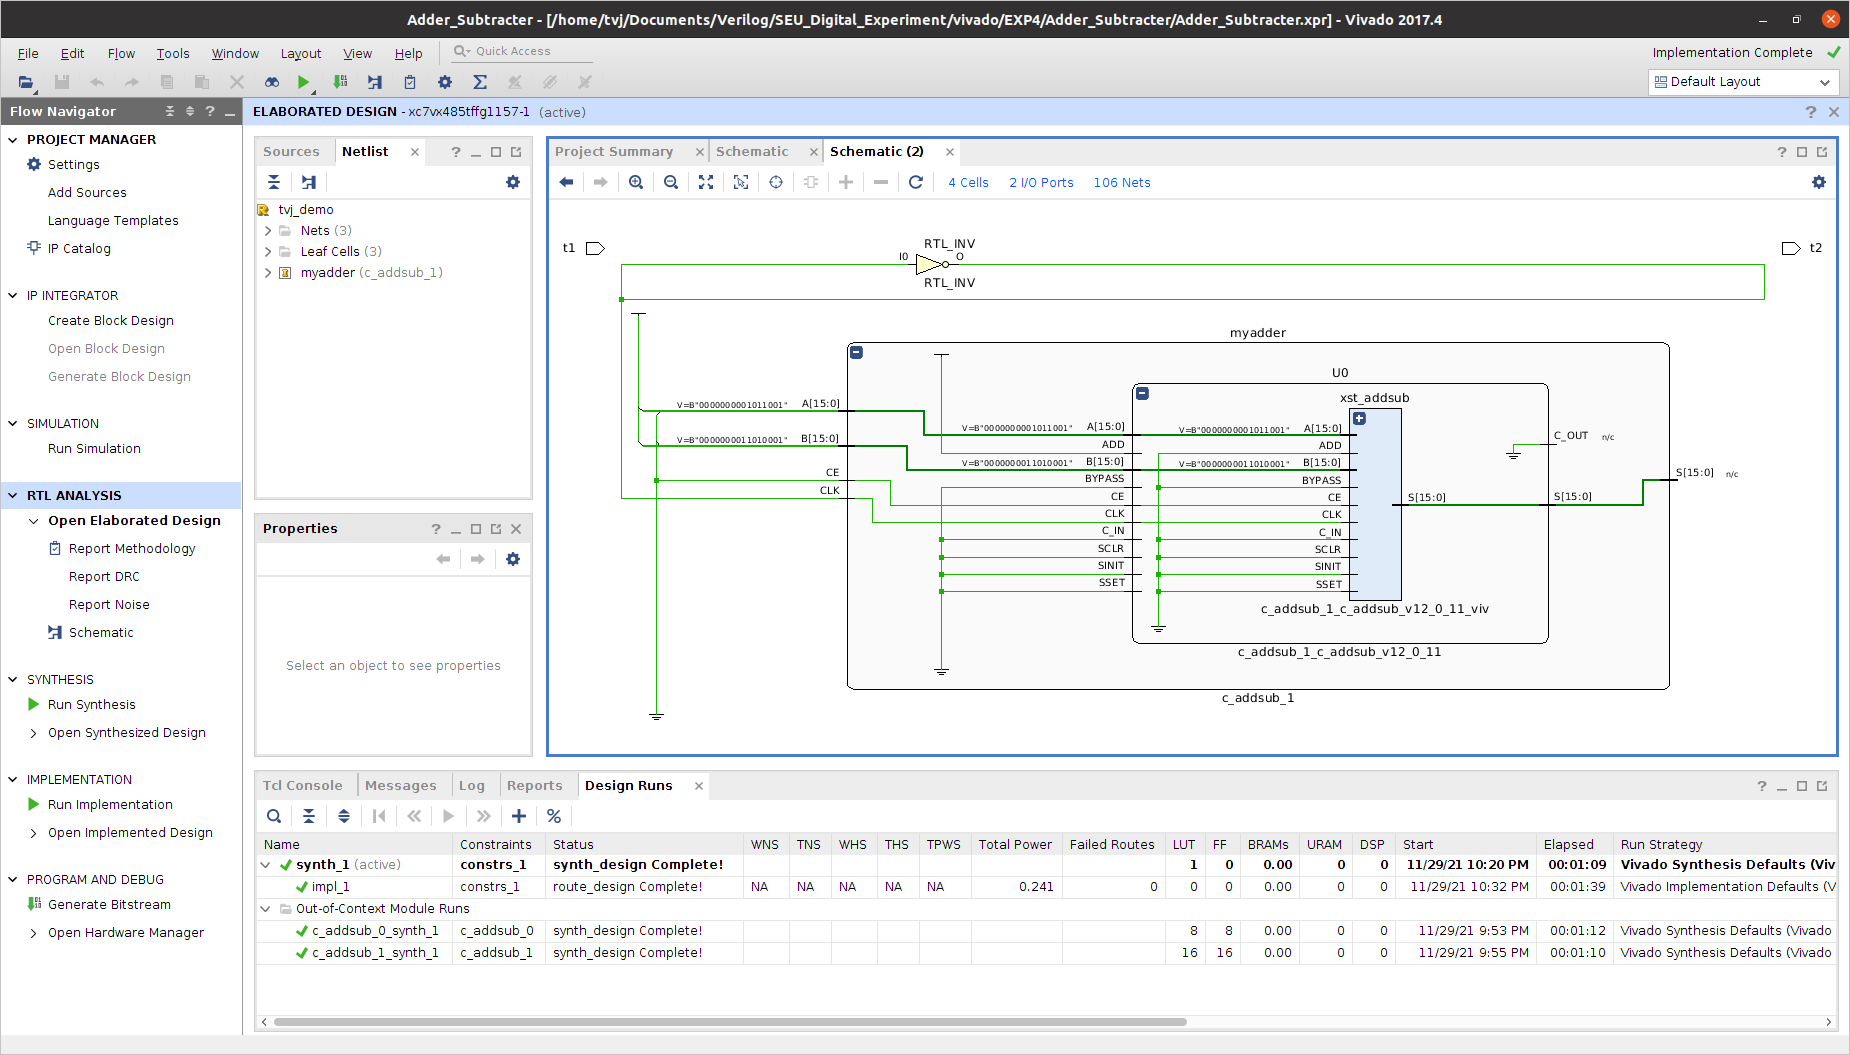
\includegraphics[width=\linewidth]{fig/IP_RTL_detailed.png}
          \caption{RTL 级电路(展开两级)}
          \label{fig:IP_RTL_detailed}
        \end{figure}

        \begin{figure}[htbp]
          \centering
          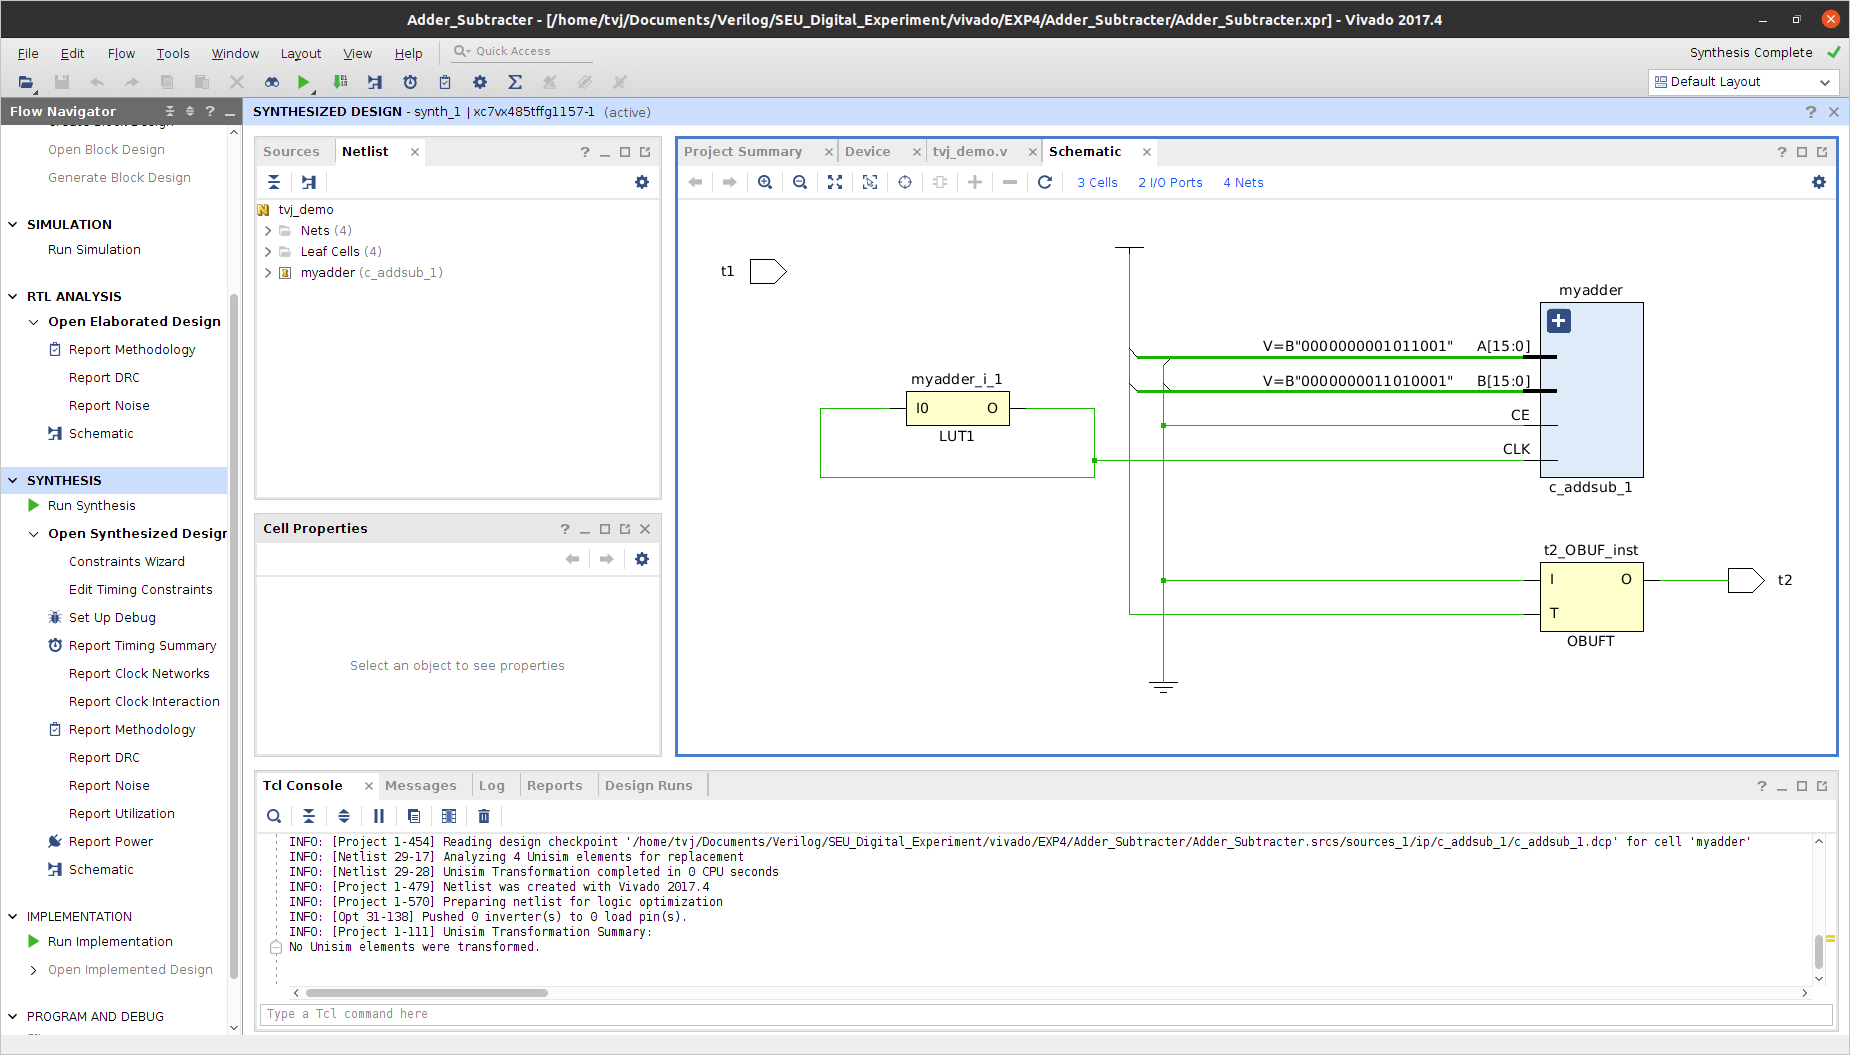
\includegraphics[width=\linewidth]{fig/IP_sys.png}
          \caption{综合电路}
          \label{fig:IP_sys}
        \end{figure}

        \clearpage
        \begin{figure}[htbp]
          \centering
          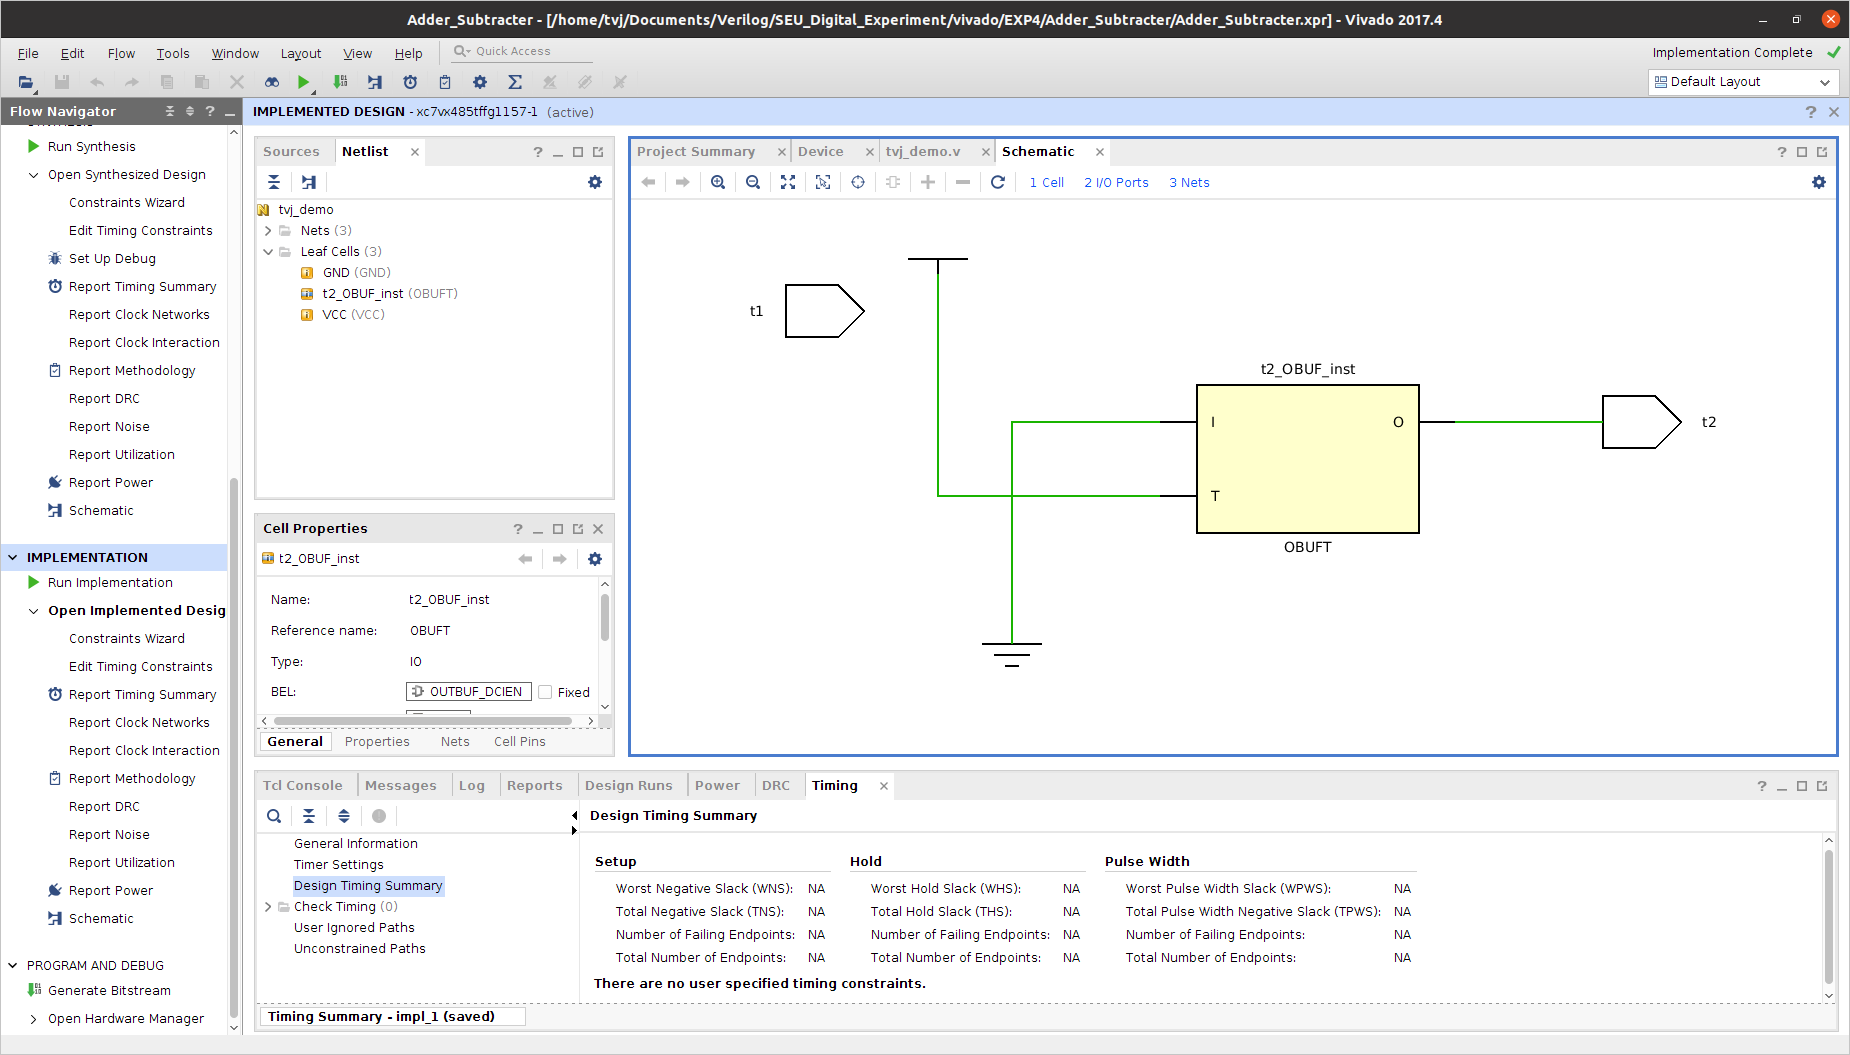
\includegraphics[width=\linewidth]{fig/IP_imp.png}
          \caption{实现电路}
          \label{fig:IP_imp}
        \end{figure}

      \subsubsection{(原理)框图设计(Block design)调用IP 核搭建}

        使用,Block Design,设计输入和输出的 port,并用鼠标连接对应的端口.
        绘图结果如图~\ref{fig:BS} 所示.
        \begin{note}{}{}
          此处我没有按照实验指导书做8位的,而是15位,因此都是 \texttt{[14:0]}.
        \end{note}

        得到的 RTL 级电路如图~\ref{fig:BS_RTL} 所示,生成的 wrapper 代码如图~\ref{fig:BS_wrapper} 所示.

        \begin{analyze}{框图设计(Block design)调用IP 核搭建}{}
          使用框图设计整体思路是比较清晰的,选择 IP 核之后设置对应的输入输出端口完成链接.
          生成出的 RTL 级电路看上去就结构清晰,此外生成的 wrapper 代码也非常易读,与使用框图设计出来的结果一致.
          这个过程其实很像软件制作的 Qt,UI 界面既可以使用代码直接完成,又可以通过拖拽的方法设置 \texttt{.ui} 文件以实现快速的设置.
        \end{analyze}
        
        \begin{figure}[htbp]
          \centering
          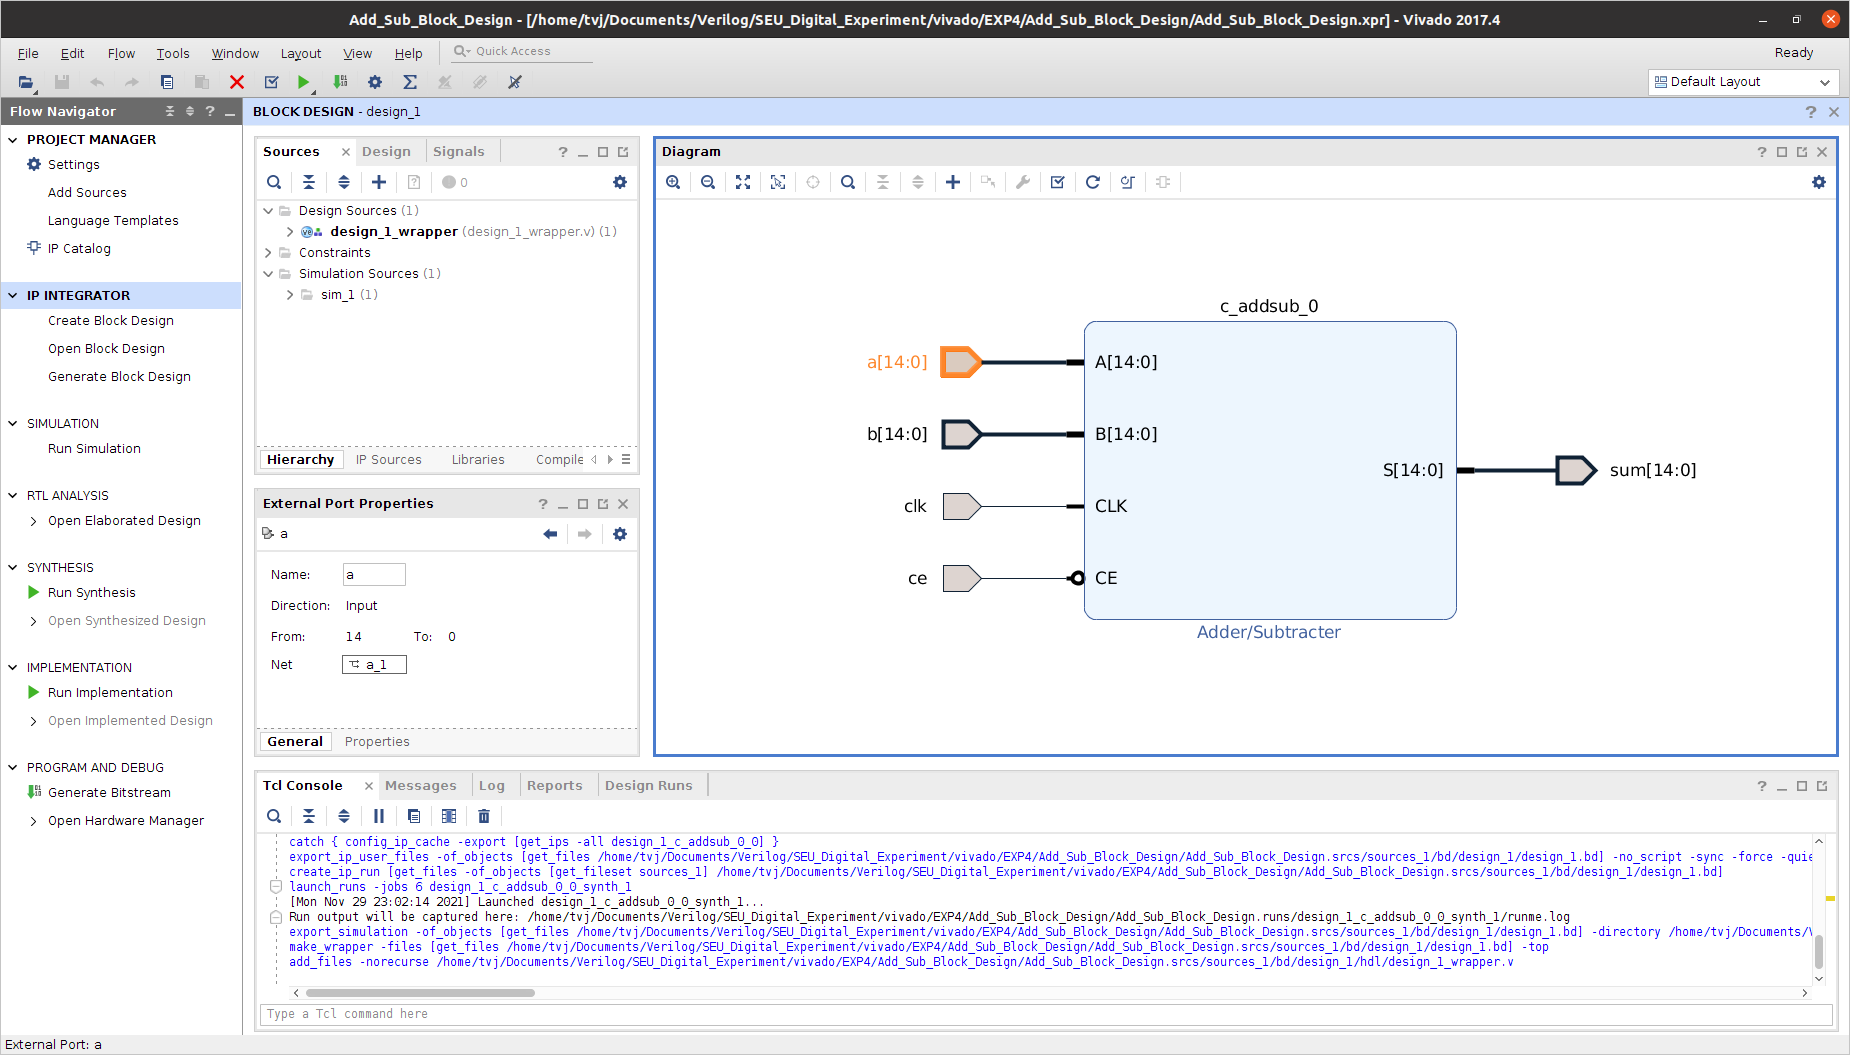
\includegraphics[width=\linewidth]{fig/BS.png}
          \caption{Block Design 界面}
          \label{fig:BS}
        \end{figure}

        \begin{figure}[htbp]
          \centering
          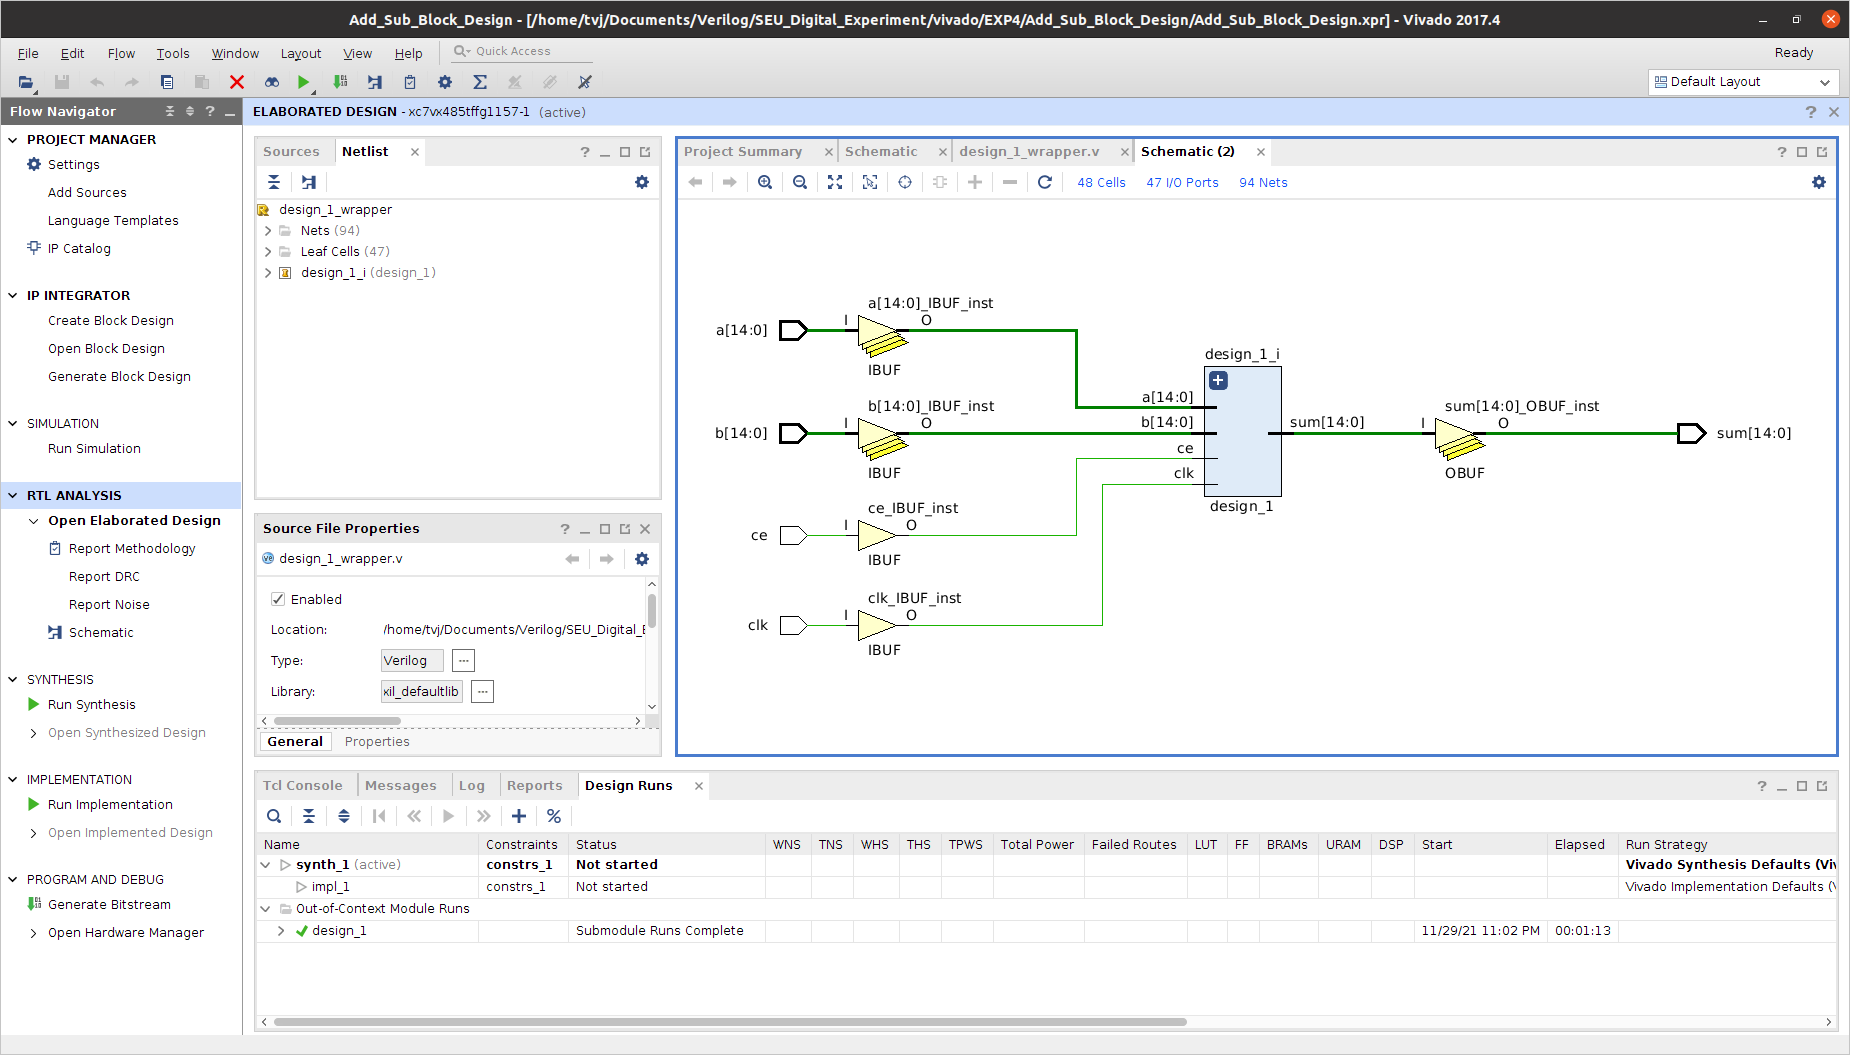
\includegraphics[width=\linewidth]{fig/BS_RTL.png}
          \caption{Block Design 的 RTL级电路}
          \label{fig:BS_RTL}
        \end{figure}

        \clearpage
        \begin{figure}[htbp]
          \centering
          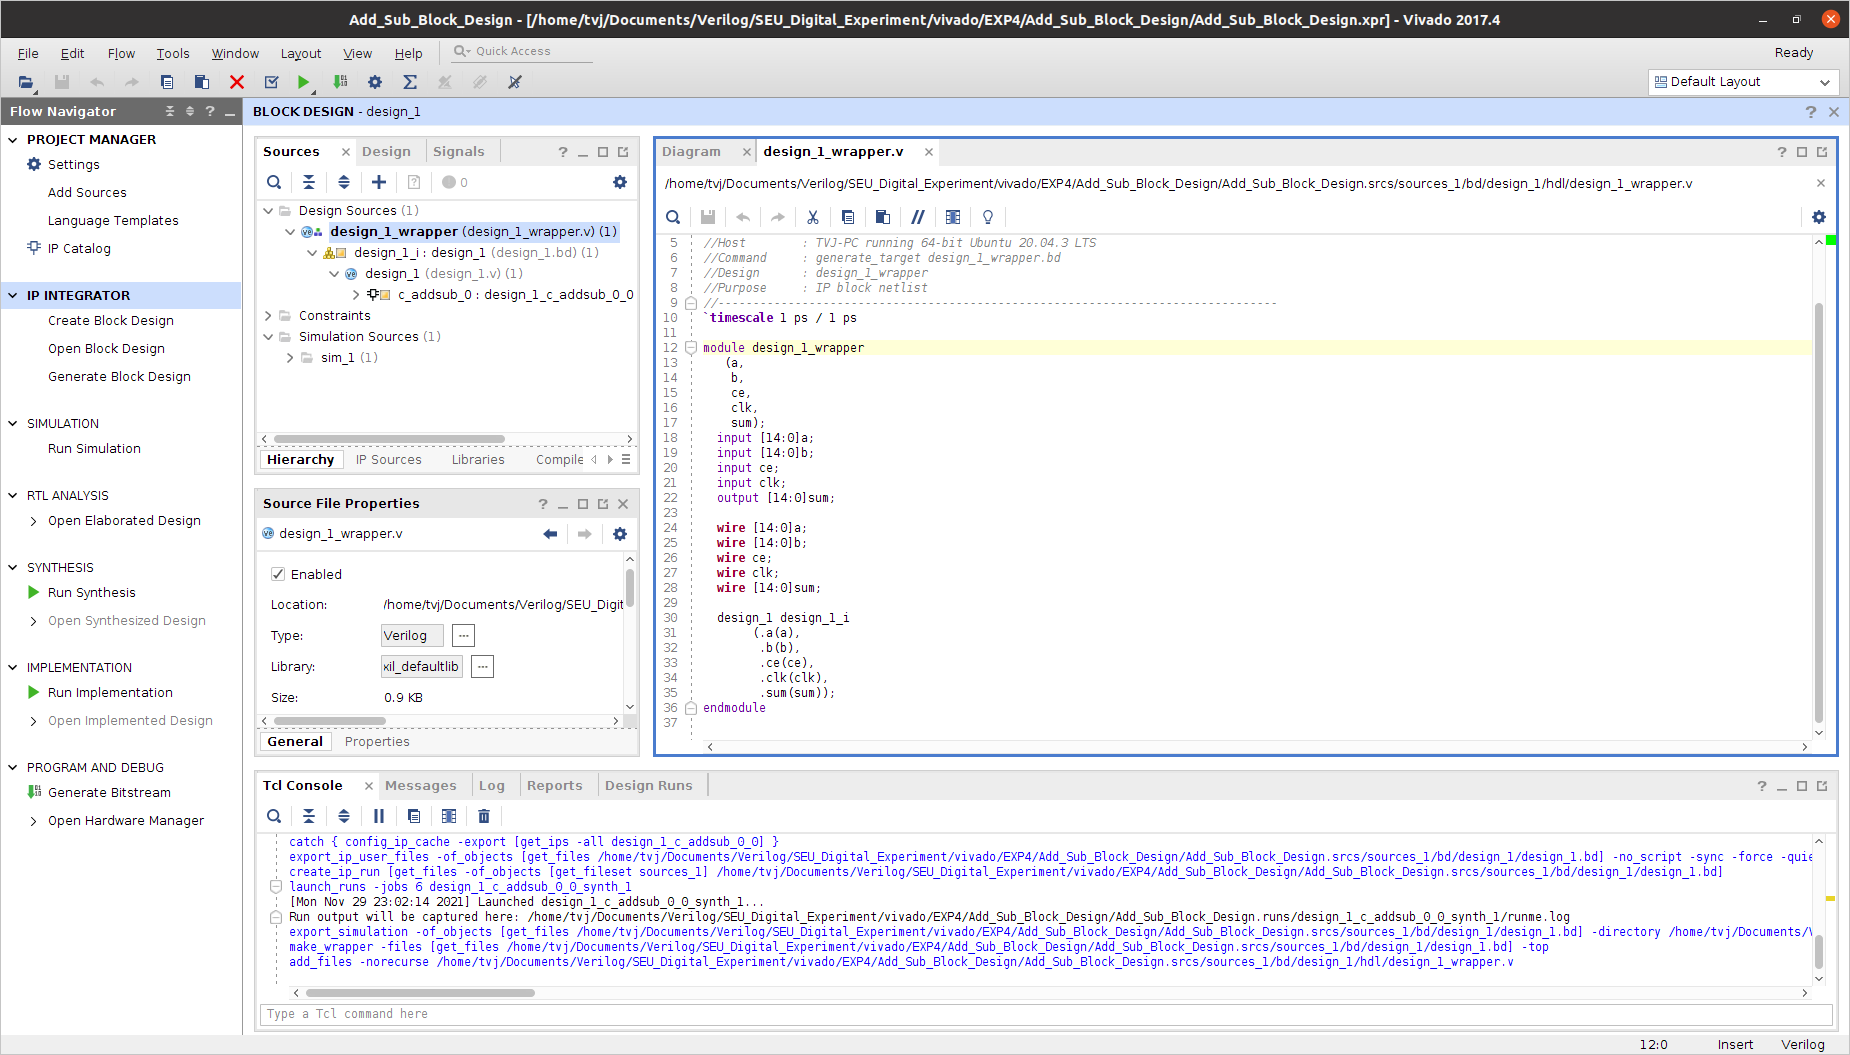
\includegraphics[width=\linewidth]{fig/BS_wrapper.png}
          \caption{Block Design 的 wrapper 代码}
          \label{fig:BS_wrapper}
        \end{figure}

      \subsection{基于 dff 的4位移位寄存器}

      带异步清零的D 触发器dff之前已经实现过了,此处代码不单独拿出来,图~\ref{fig:DFF_RTL} 是其RTL级电路图.
      
      4位移位寄存器 的核心实现代码如下.
      \begin{lstlisting}[language=verilog]
module ShiftRegister(C, L, RTL, R, D, Q, nQ);
  parameter n = 4;
  reg [n - 1:0] Dm;
  input wire C, L, RTL, R;
  input wire [n - 1:0] D;
  output wire [n - 1:0] Q;
  output wire [n - 1:0] nQ;

  always@(posedge C or posedge L)
  begin
    if(R)
      assign Dm = 0;
    else if (L == 0)
      begin
        if (RTL == 1)
          assign Dm = {Q[n - 2:0], D[0]}; // shift right
        else
          assign Dm = {D[n - 1], Q[n - 1:1]};
      end
    else
      begin
        assign Dm = {D[n - 1:0]};
      end
  end

  genvar i;
  generate for (i = 0; i < n; i = i + 1)
    DFlipFlop dff(.C(C), .D(Dm[i]), .Q(Q[i]), .nQ(nQ[i]));
  endgenerate
endmodule
      \end{lstlisting}

      \begin{analyze}{}{}
        实现IP核封装的方式类似上一个实验内容,总体感觉在使用上区别不大,都是较为自然的,正如 C++ 一样进行一个较为完成的类封装.

        4位移位寄存器代码参考:\url{https://github.com/AliRezaBeigy/ShiftRegister}.
      \end{analyze}

      \begin{figure}[htbp]
        \centering
        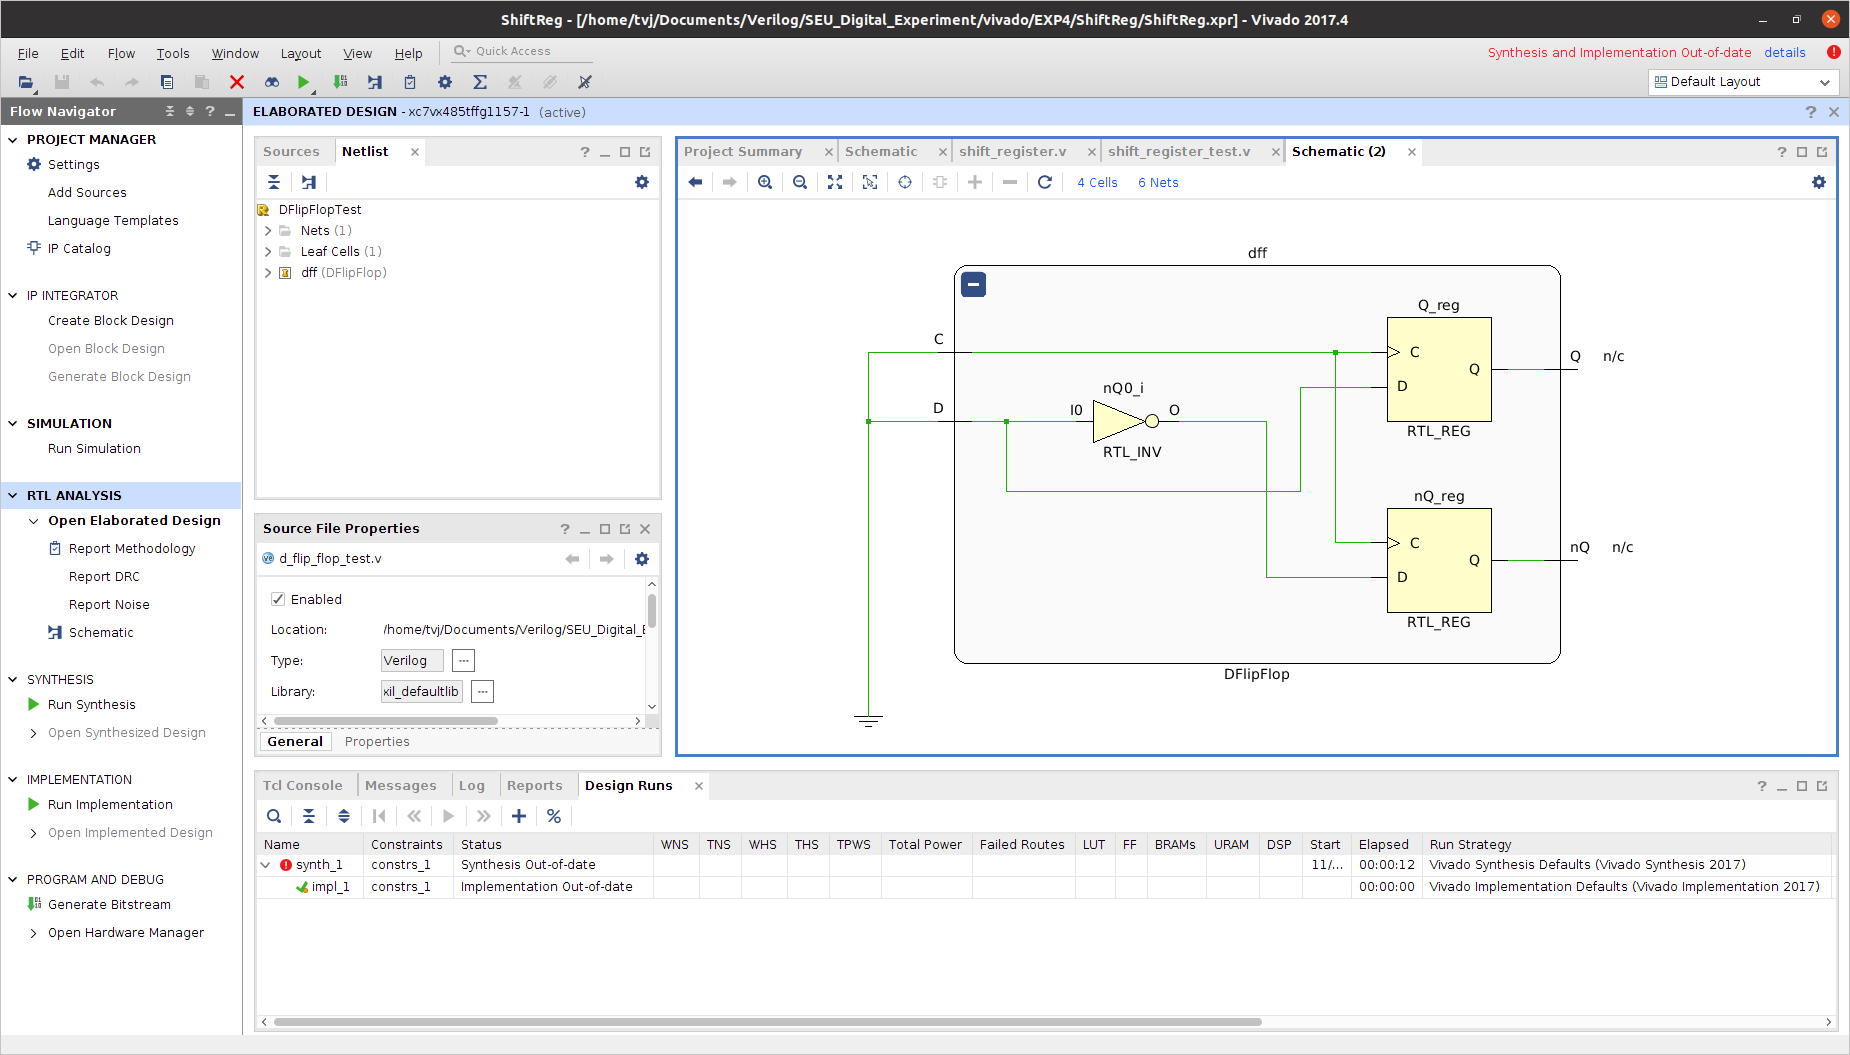
\includegraphics[width=\linewidth]{fig/DFF_RTL.png}
        \caption{4位移位寄存器的行为仿真图}
        \label{fig:DFF_RTL}
      \end{figure}

      \clearpage
      \begin{figure}[htbp]
        \centering
        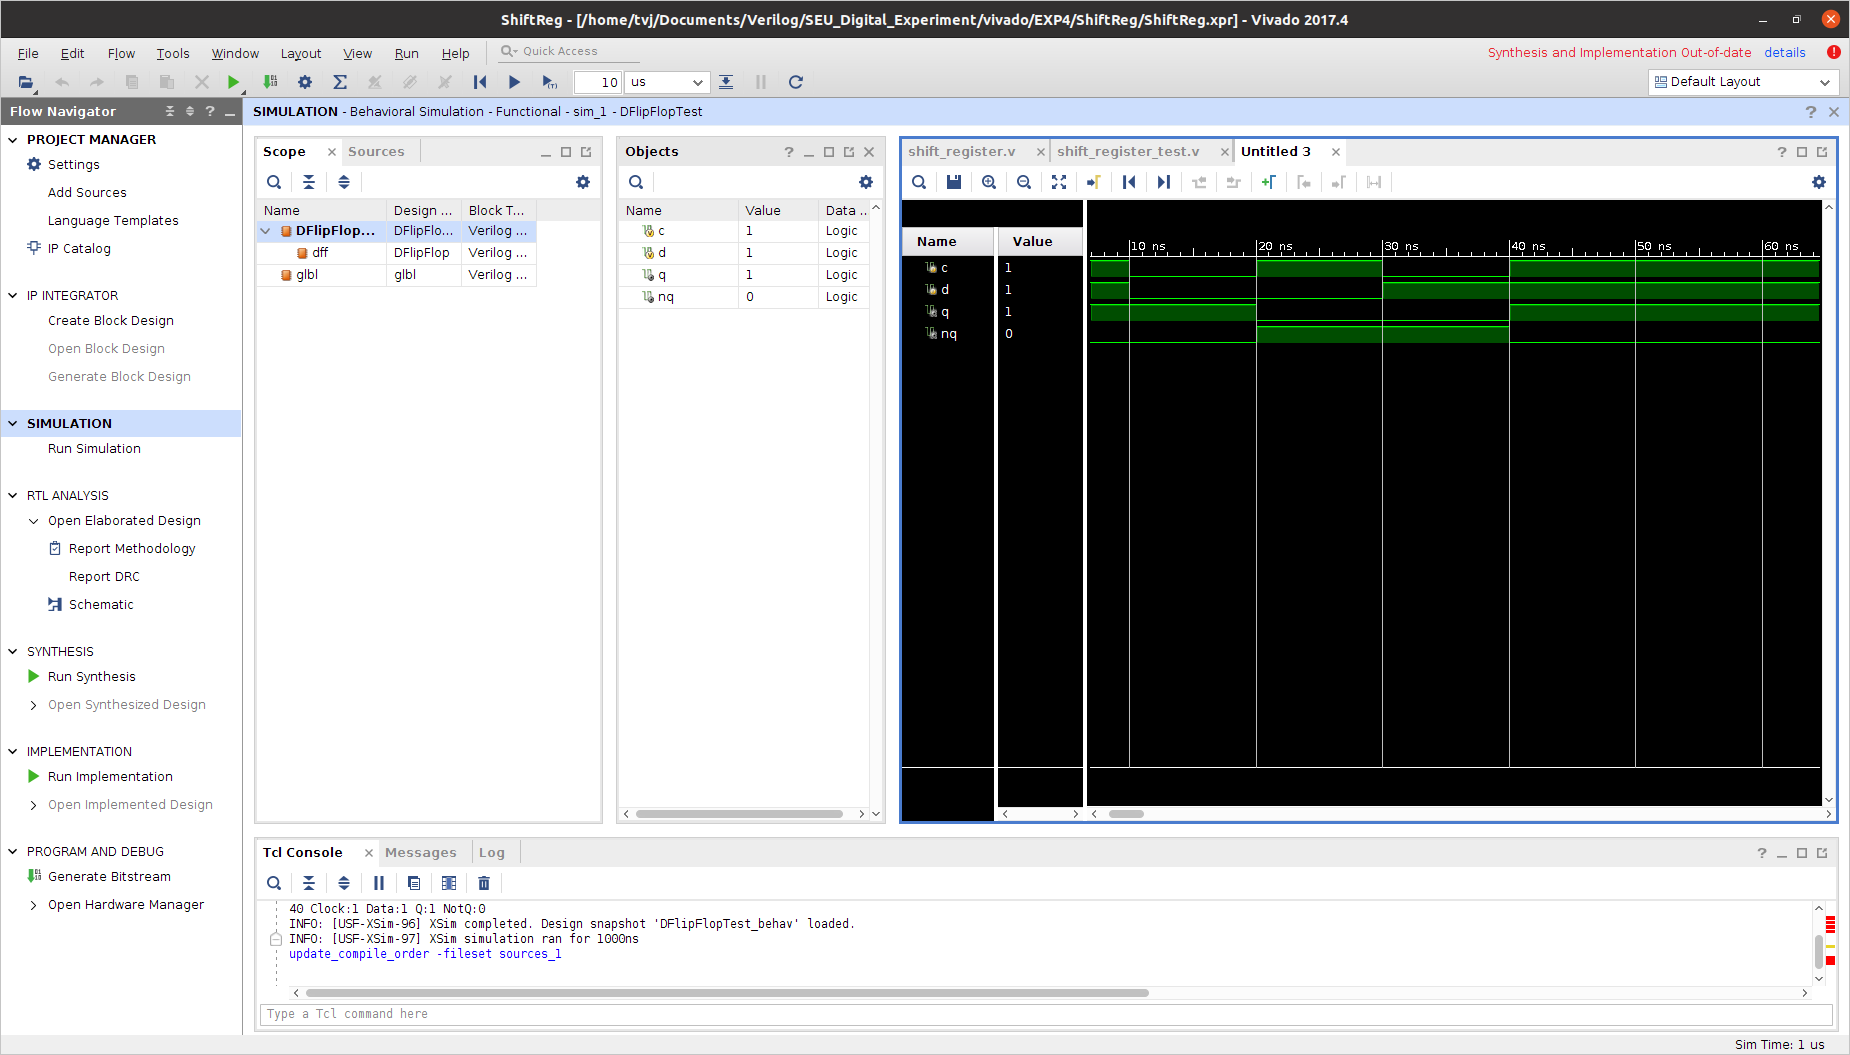
\includegraphics[width=\linewidth]{fig/Reg_simu.png}
        \caption{4位移位寄存器的行为仿真图}
        \label{fig:Reg_simu}
      \end{figure}

    \subsection{Altera 的使用}

      首先,搭建图~\ref{fig:Altera_1} 的电路图,行为仿真得到图~\ref{fig:Altera_2} 的结果,验证了累加器的工作方式.
      接下来需要配置引脚文件,由于实验指导书~\cite{guide} 附带的代码没有提供银角文件,我们需要自己设计,这个过程 \cite{guide} 上也没有介绍,我们通过学习网上资料,完成了如下的工作.
      首先,需要如图~\ref{fig:Altera_3} 选择我们使用的开发板型号:\texttt{Cyclone EP1C6Q240C8},再设置每个引脚的连接(如图~\ref{fig:Altera_4}),这个过程会十分繁琐,
      设置好部分引脚的结果如图~\ref{fig:Altera_5} 所示,右边的引脚伤未完成分配.
      如果引脚是已经写好的,可以用图~\ref{fig:Altera_7} 的方法导入(但是很不幸,提供的材料没有,选择的文件都是我们自己刚新建的那一个).


      \begin{analyze}{}{}
        \begin{itemize}
          \item 图~\ref{fig:Altera_2} 中可以看到进位信息(不过在屏幕上一动起来效果会更好一些),对于累加器的理解有了更深入的理解;
          \item 通过LD/CNT 控制\texttt{A7..0}
          可以在每个时钟周期自加一或者接受来自数据总线的数据;
          \item 由于引脚分配过于困难,我们在后面采用了提供的程序来做烧录板子的工作.
        \end{itemize}
      \end{analyze}

      \newpage
      \begin{figure}[htbp]
        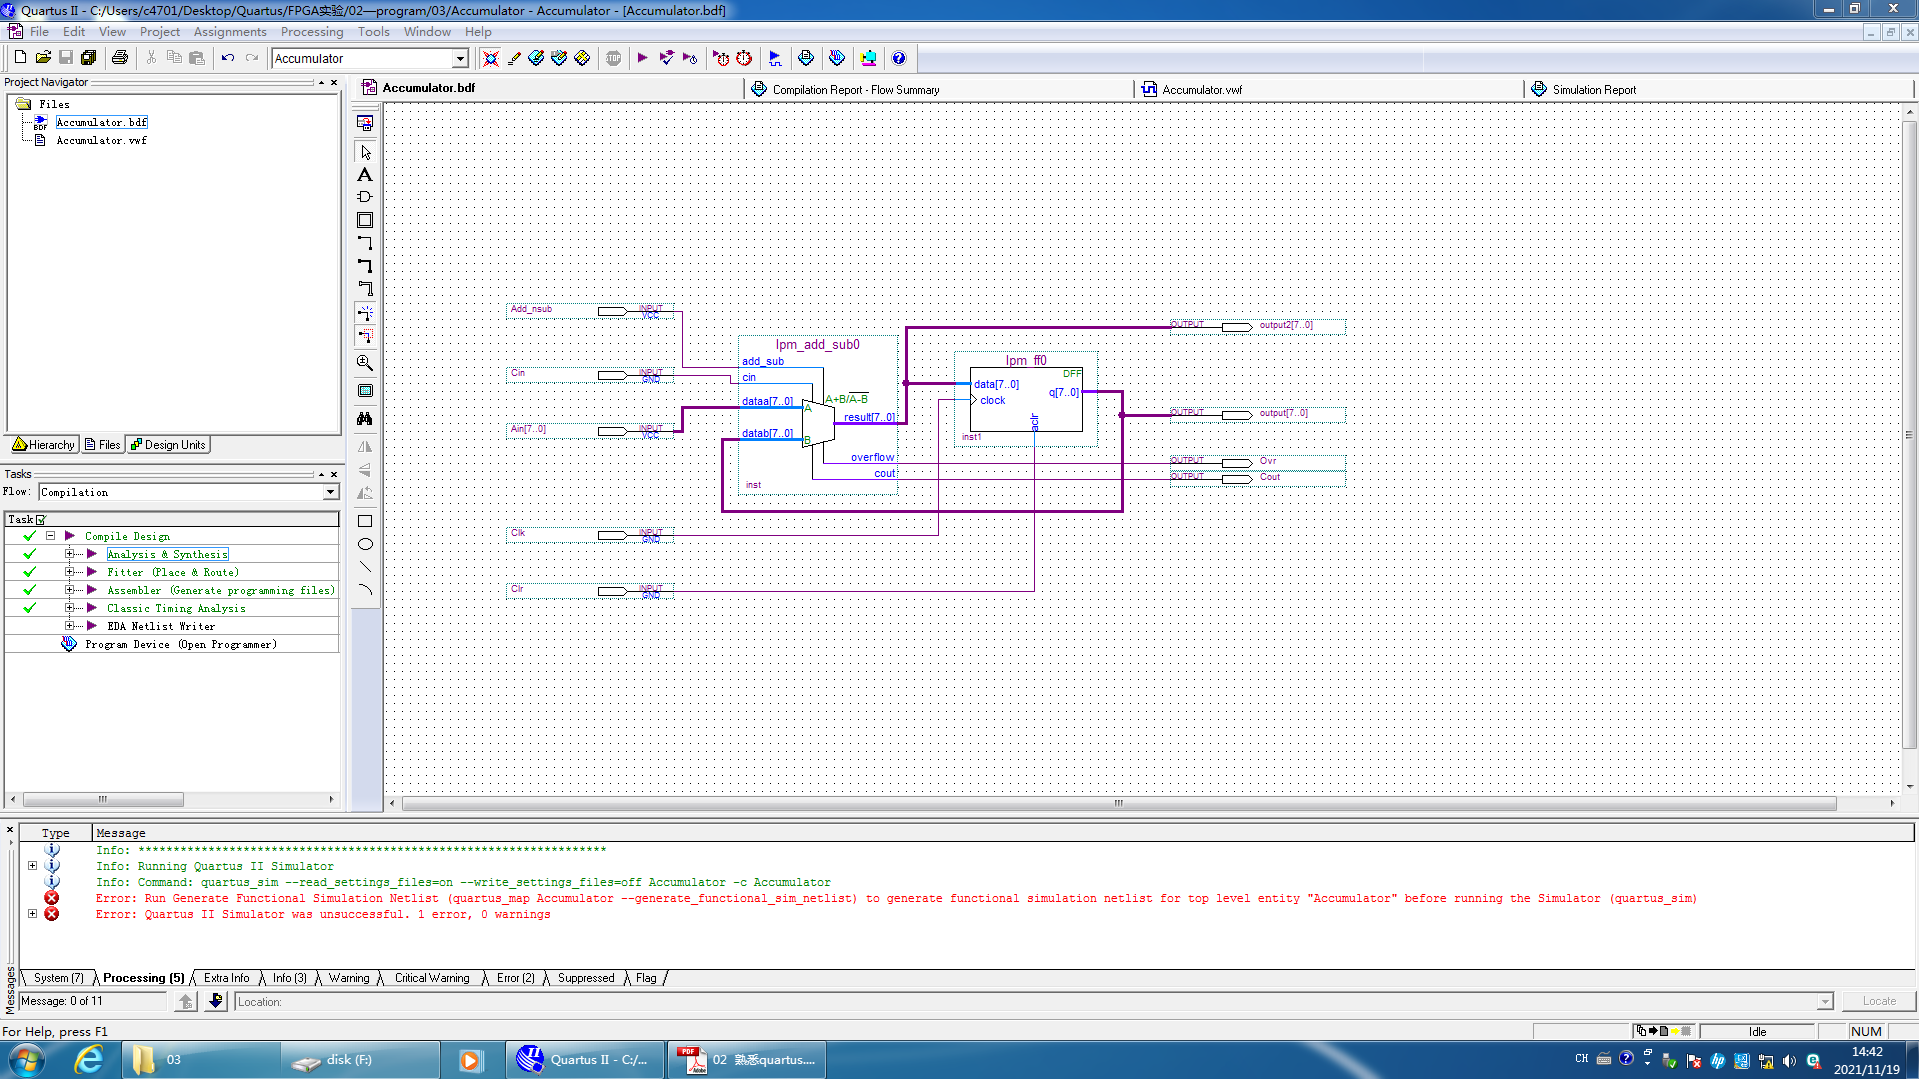
\includegraphics[width=\linewidth]{fig/Altera/1.PNG}
        \caption{基于LPM 库的累加器电路原理图}
        \label{fig:Altera_1}
      \end{figure}

      \begin{figure}[h!]
        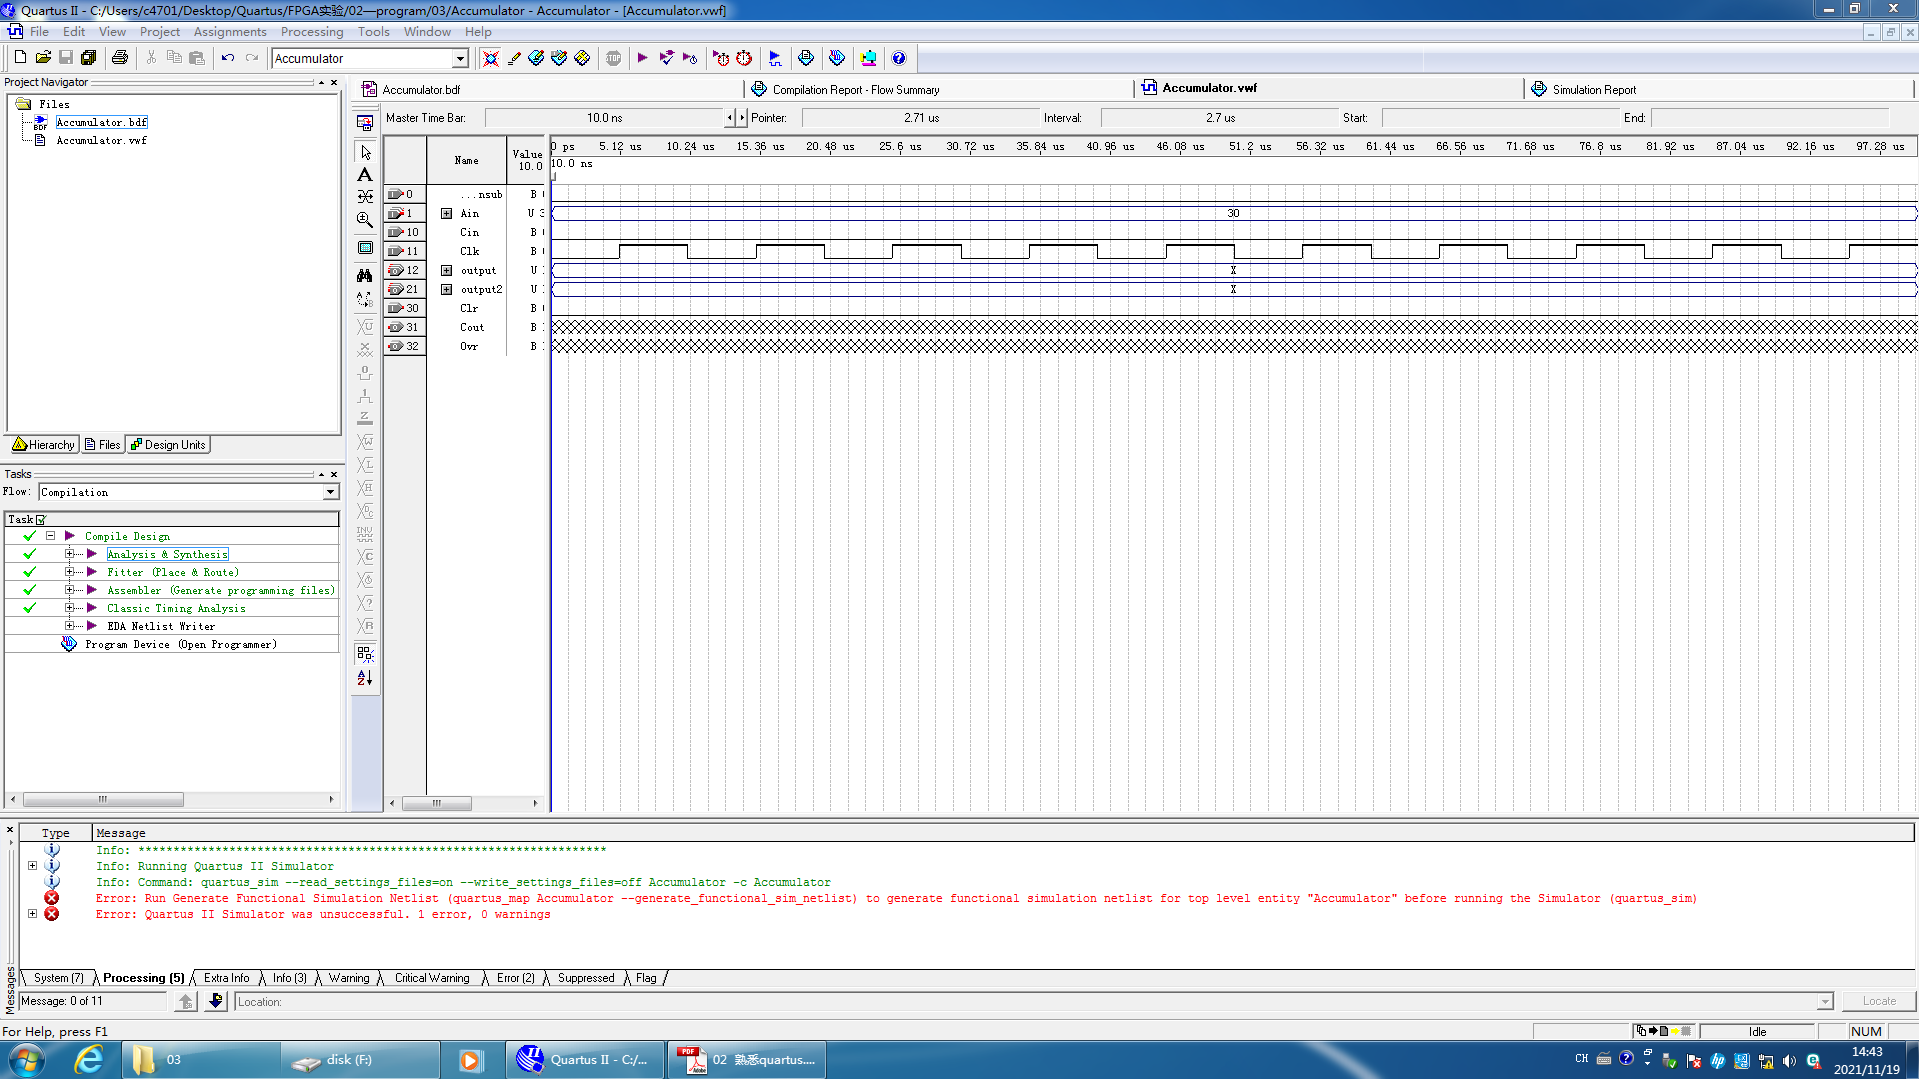
\includegraphics[width=\linewidth]{fig/Altera/2.PNG}
        \caption{仿真结果}
        \label{fig:Altera_2}
      \end{figure}

      \newpage
      \begin{figure}[htbp]
        \centering
        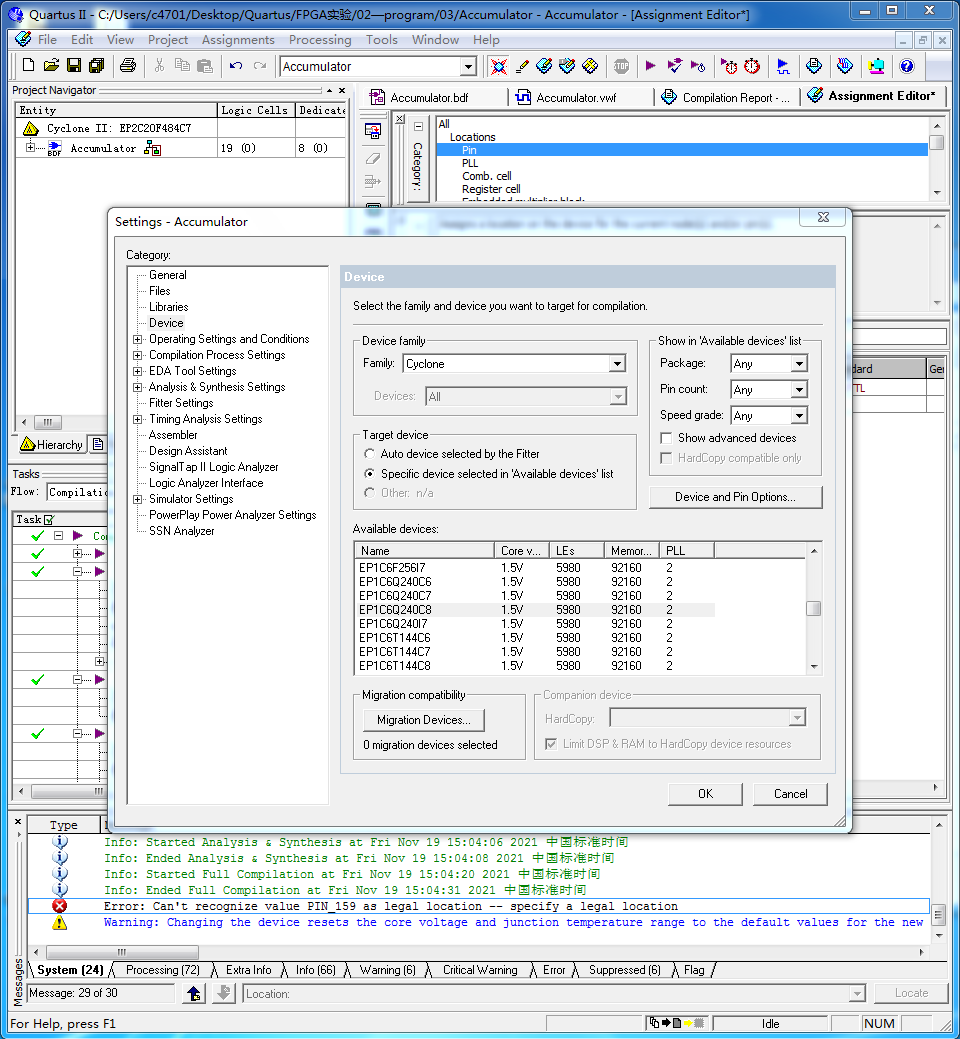
\includegraphics[width=.5\linewidth]{fig/Altera/3.PNG}
        \caption{选择仪器型号}
        \label{fig:Altera_3}
      \end{figure}

      \begin{figure}[h!]
        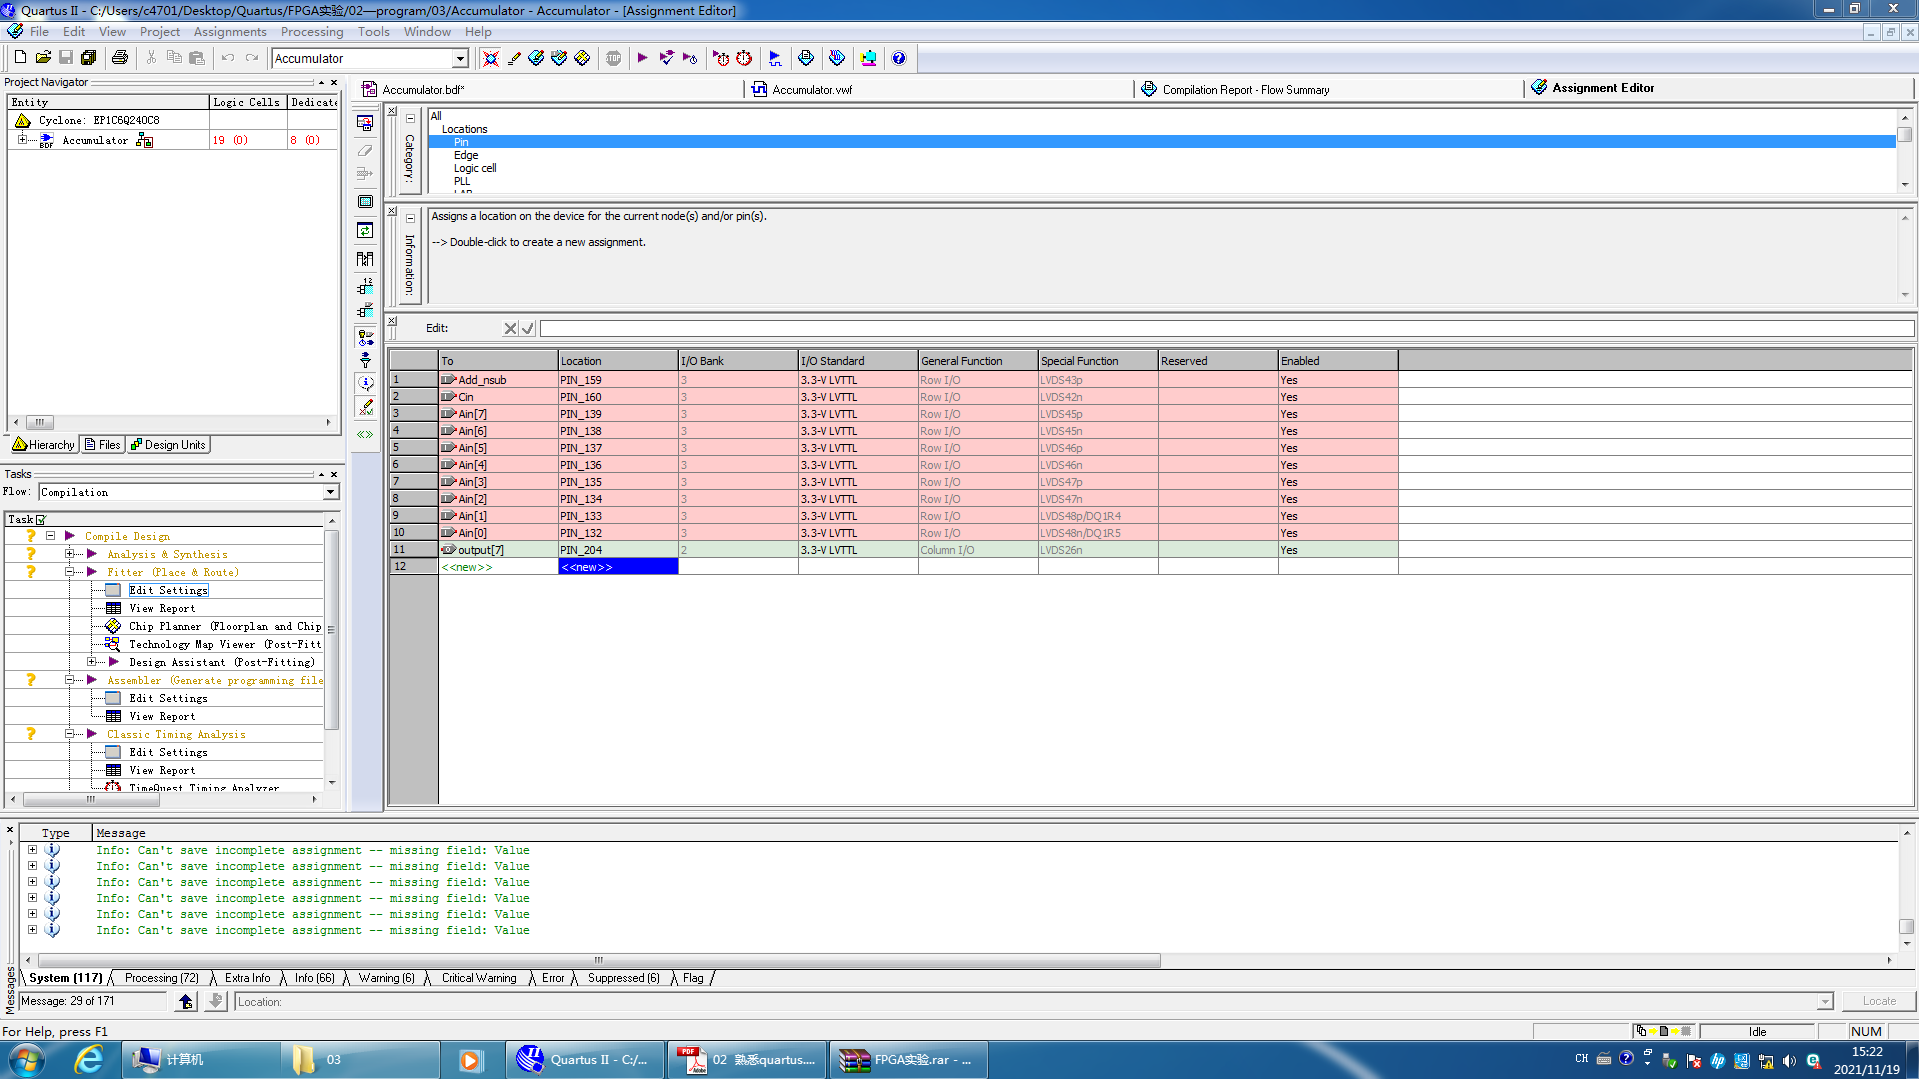
\includegraphics[width=\linewidth]{fig/Altera/6.PNG}
        \caption{设置引脚}
        \label{fig:Altera_4}\label{fig:Altera_6}
      \end{figure}

      \newpage
      \begin{figure}[htbp]
        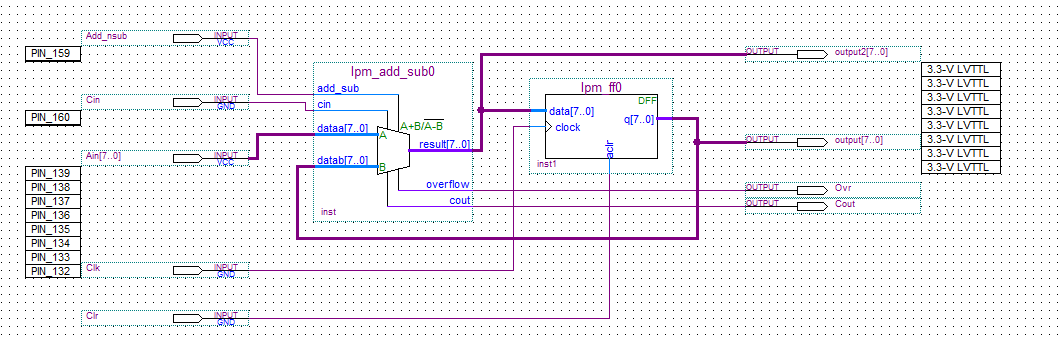
\includegraphics[width=\linewidth]{fig/Altera/5.PNG}
        \caption{设置引脚的结果}
        \label{fig:Altera_5}
      \end{figure}

      \begin{figure}[h!]
        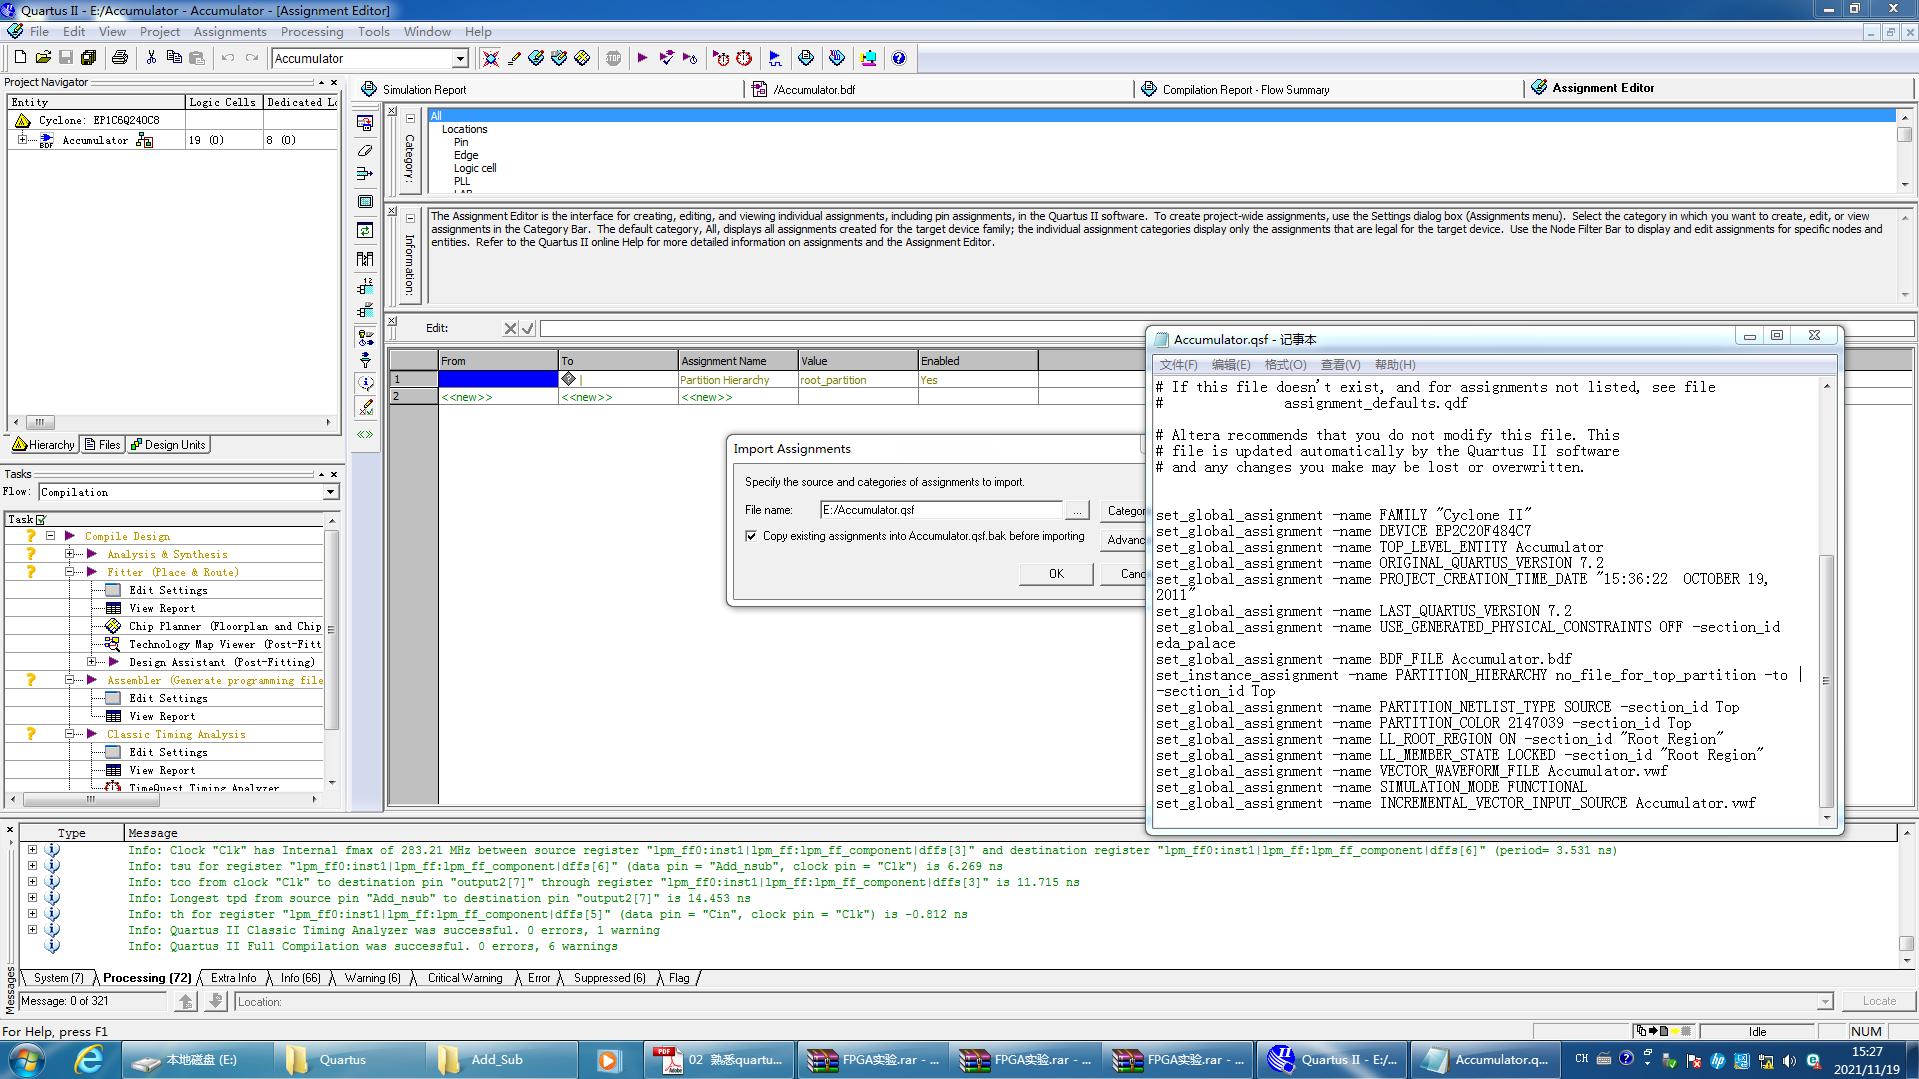
\includegraphics[width=\linewidth]{fig/Altera/7.PNG}
        \caption{导入引脚配置文件}
        \label{fig:Altera_7}
      \end{figure}

      % ======
      \emptyline

      我们以提供的项目为蓝本,设计了 \texttt{74138} 和灯测试及测试单元的电路并进行了测试,
      图~\ref{fig:Altera_8} 是\texttt{74138} 电路设计图,图~\ref{fig:Altera_11} 是灯测试的电路,图~\ref{fig:Altera_12} 是测试模块的电路.
      以图~\ref{fig:Altera_9} 的方式将项目烧录至开发板中,
      实现了预计的效果,主要是对整个开发的流程有了更加深入的了解,
      最后图~\ref{fig:Altera_result} 是实现的效果.

      \begin{analyze}{}{}
        整个过程较为复杂且中间的许多步骤都需要较为仔细的学习,
        而这次实验时间有限,主要目的是做一个大致的了解,对与整个开发流程有一个印象.
      \end{analyze}

      \begin{figure}[htbp]
        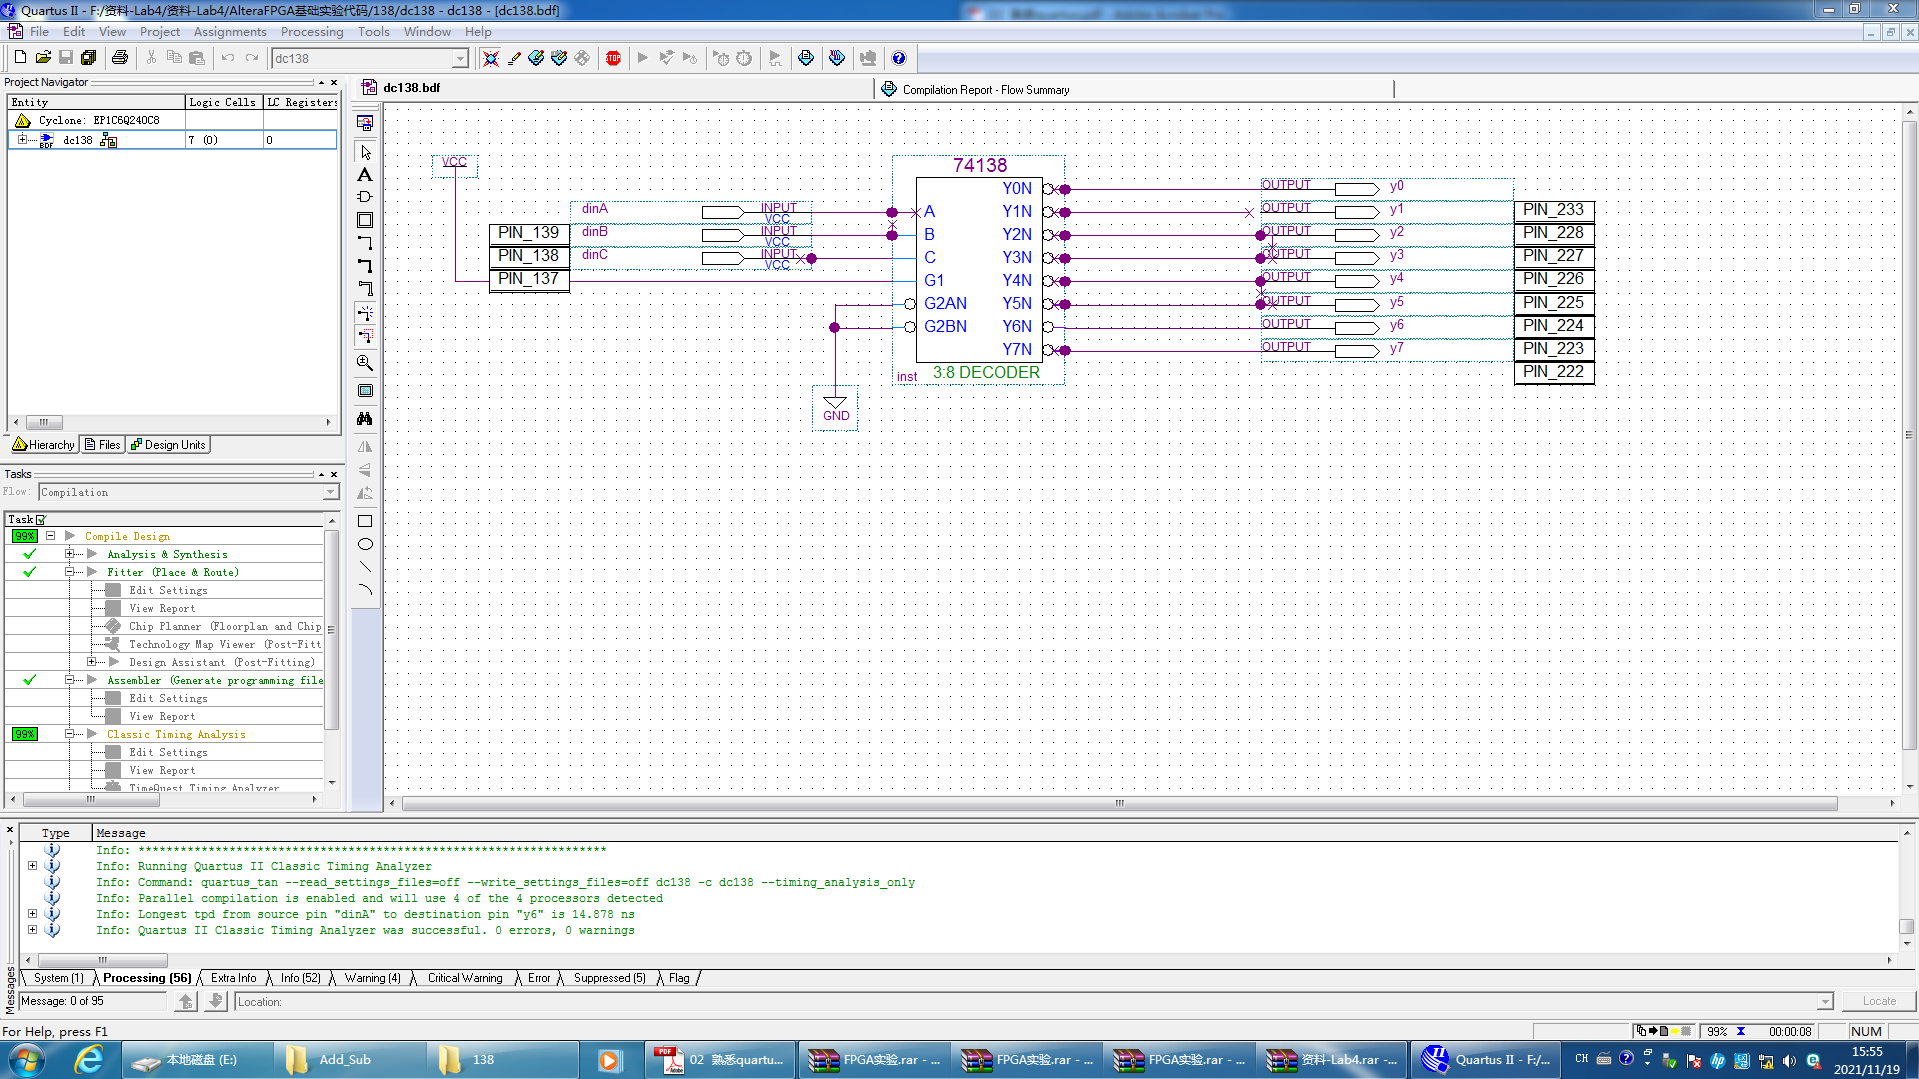
\includegraphics[width=\linewidth]{fig/Altera/8.PNG}
        \caption{74138 电路设计}
        \label{fig:Altera_8}
      \end{figure}

      \begin{figure}[htbp]
        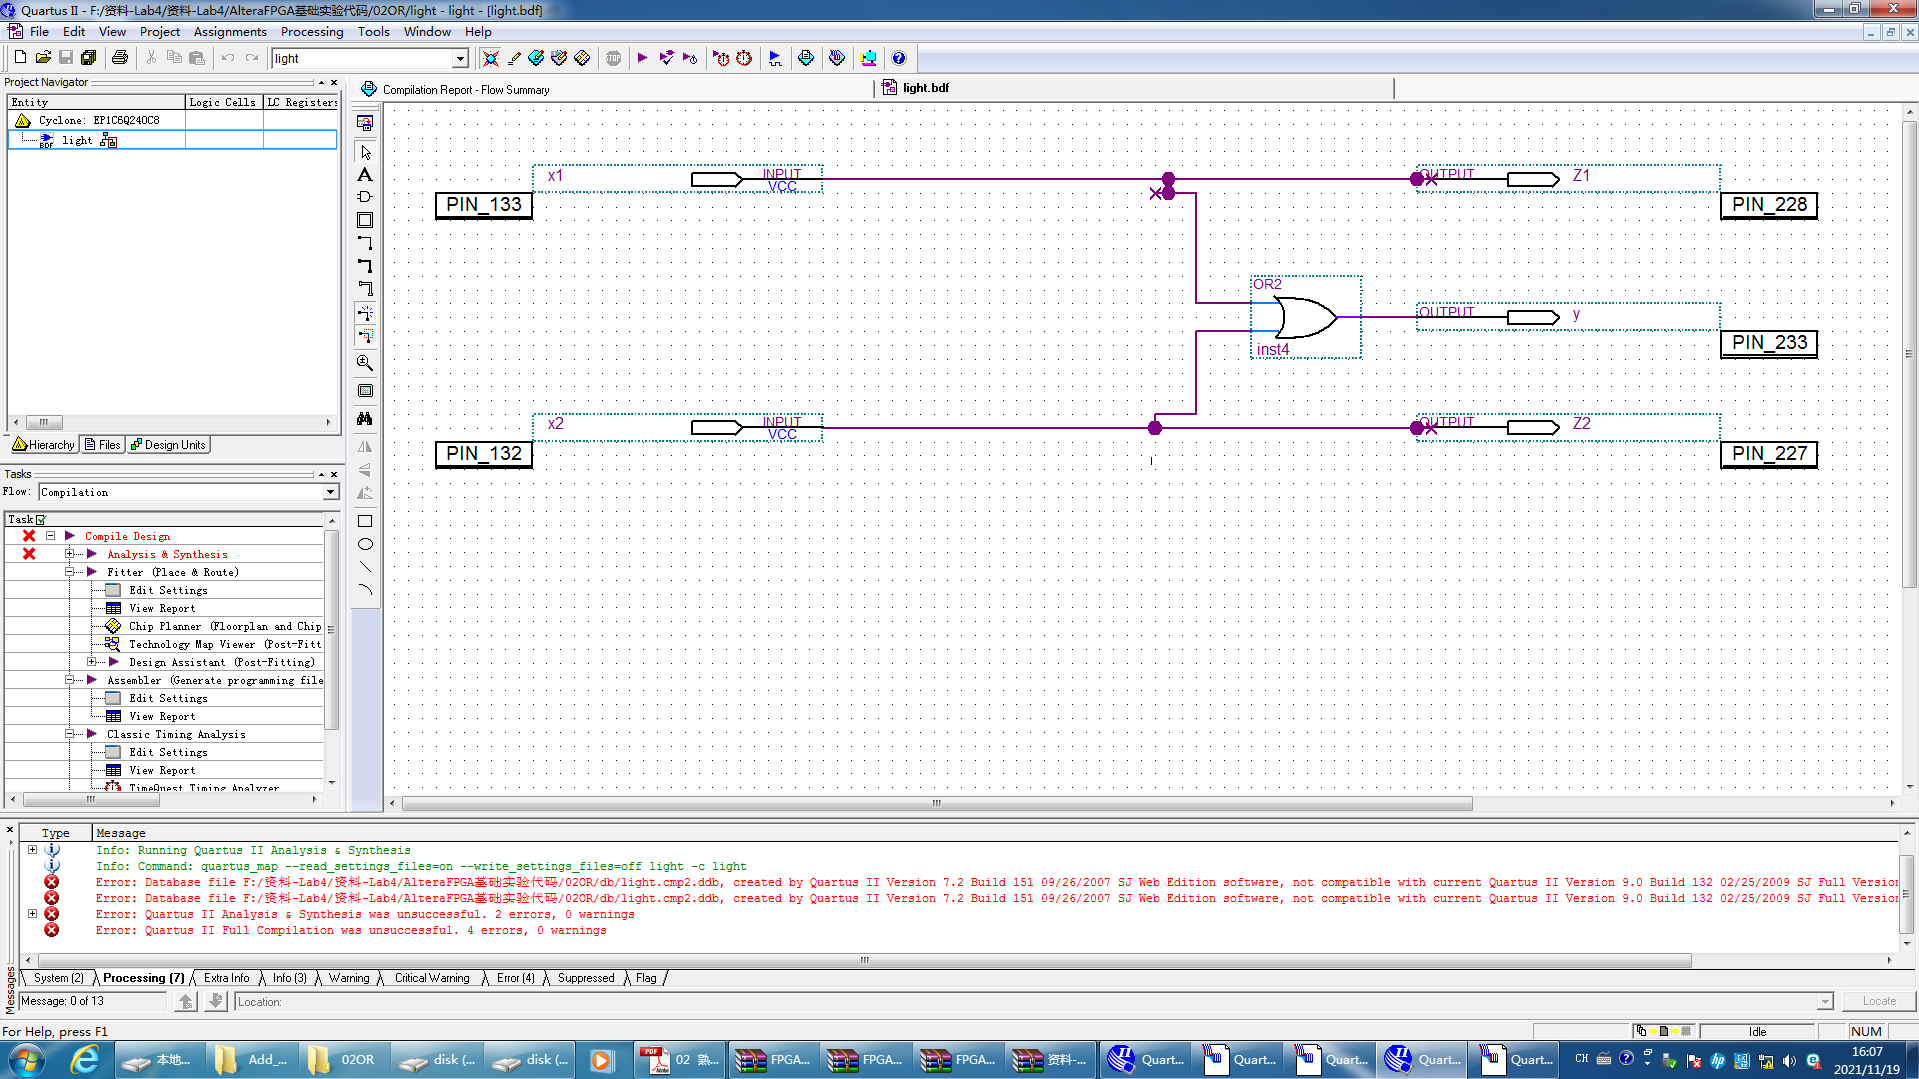
\includegraphics[width=\linewidth]{fig/Altera/11.PNG}
        \caption{灯测试电路设计}
        \label{fig:Altera_11}
      \end{figure}

      \begin{figure}[htbp]
        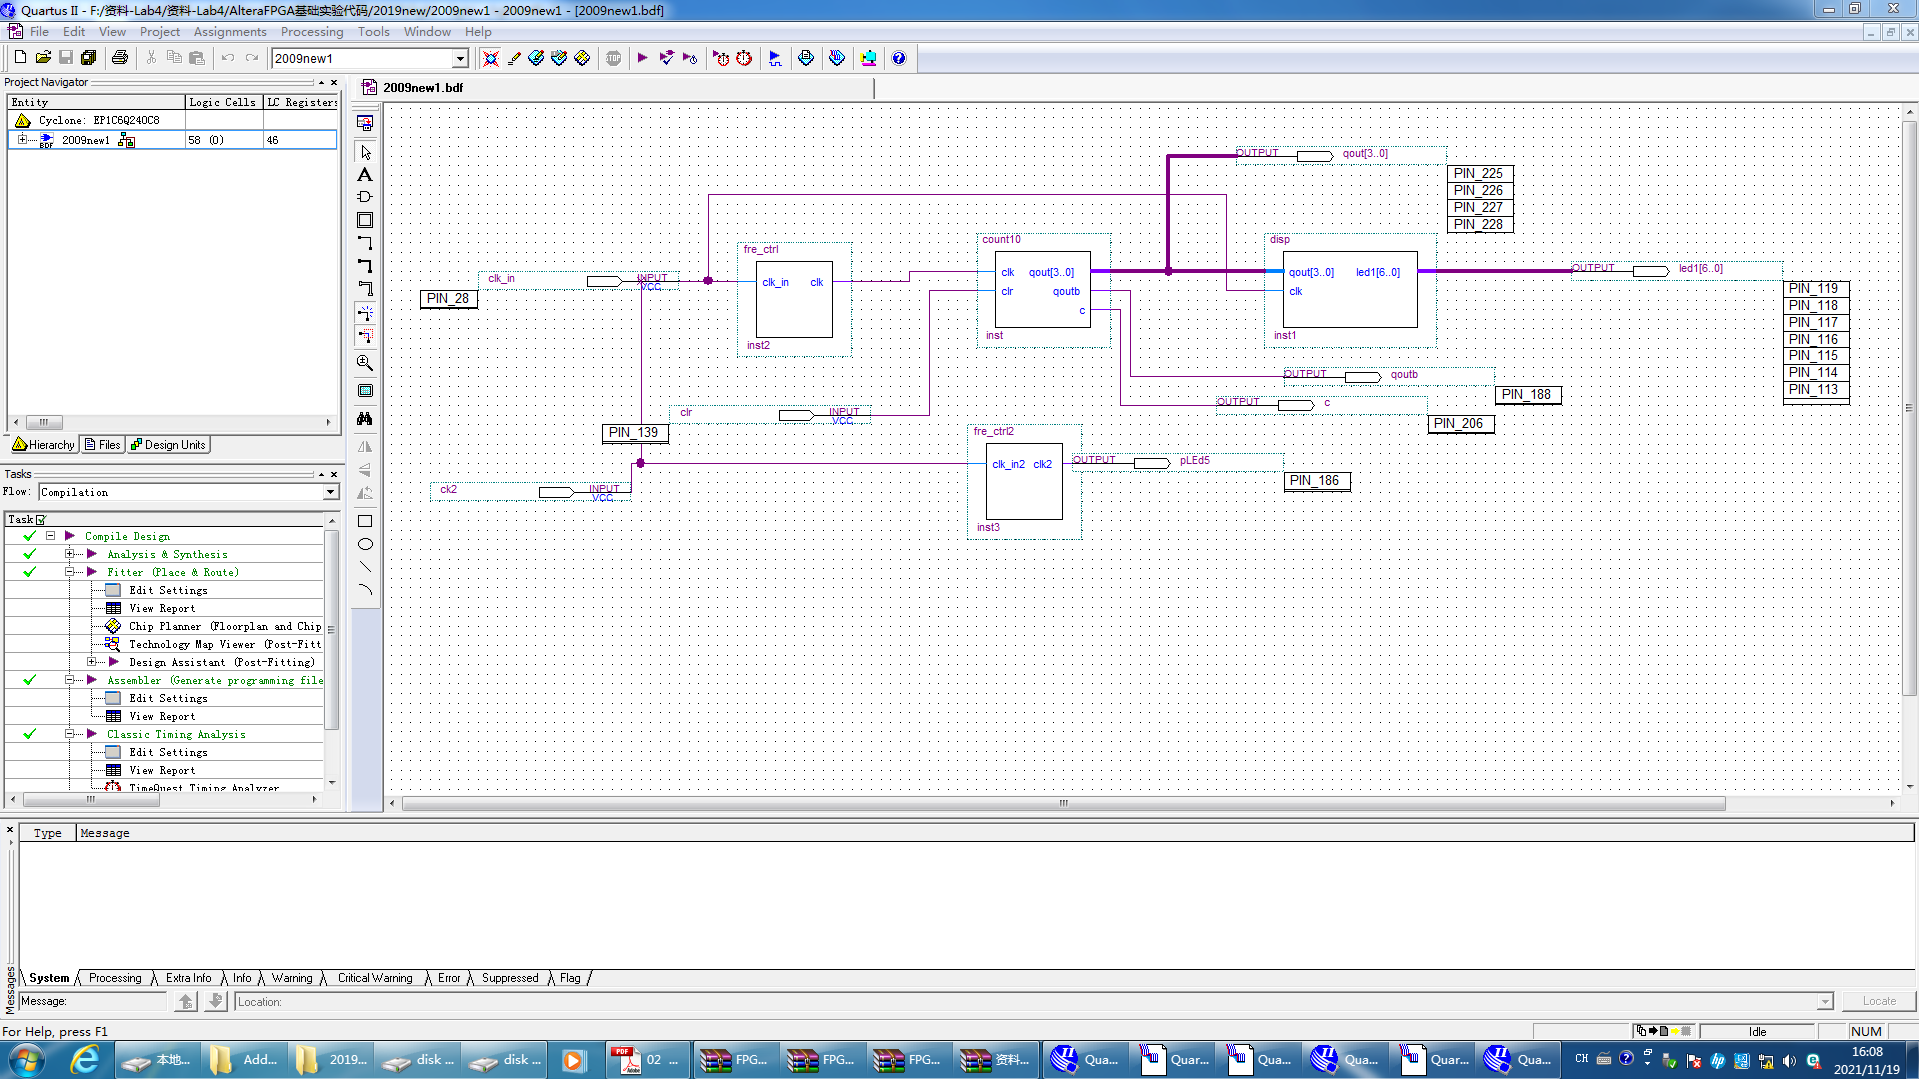
\includegraphics[width=\linewidth]{fig/Altera/12.PNG}
        \caption{测试设计}
        \label{fig:Altera_12}
      \end{figure}

      \begin{figure}[htbp]
        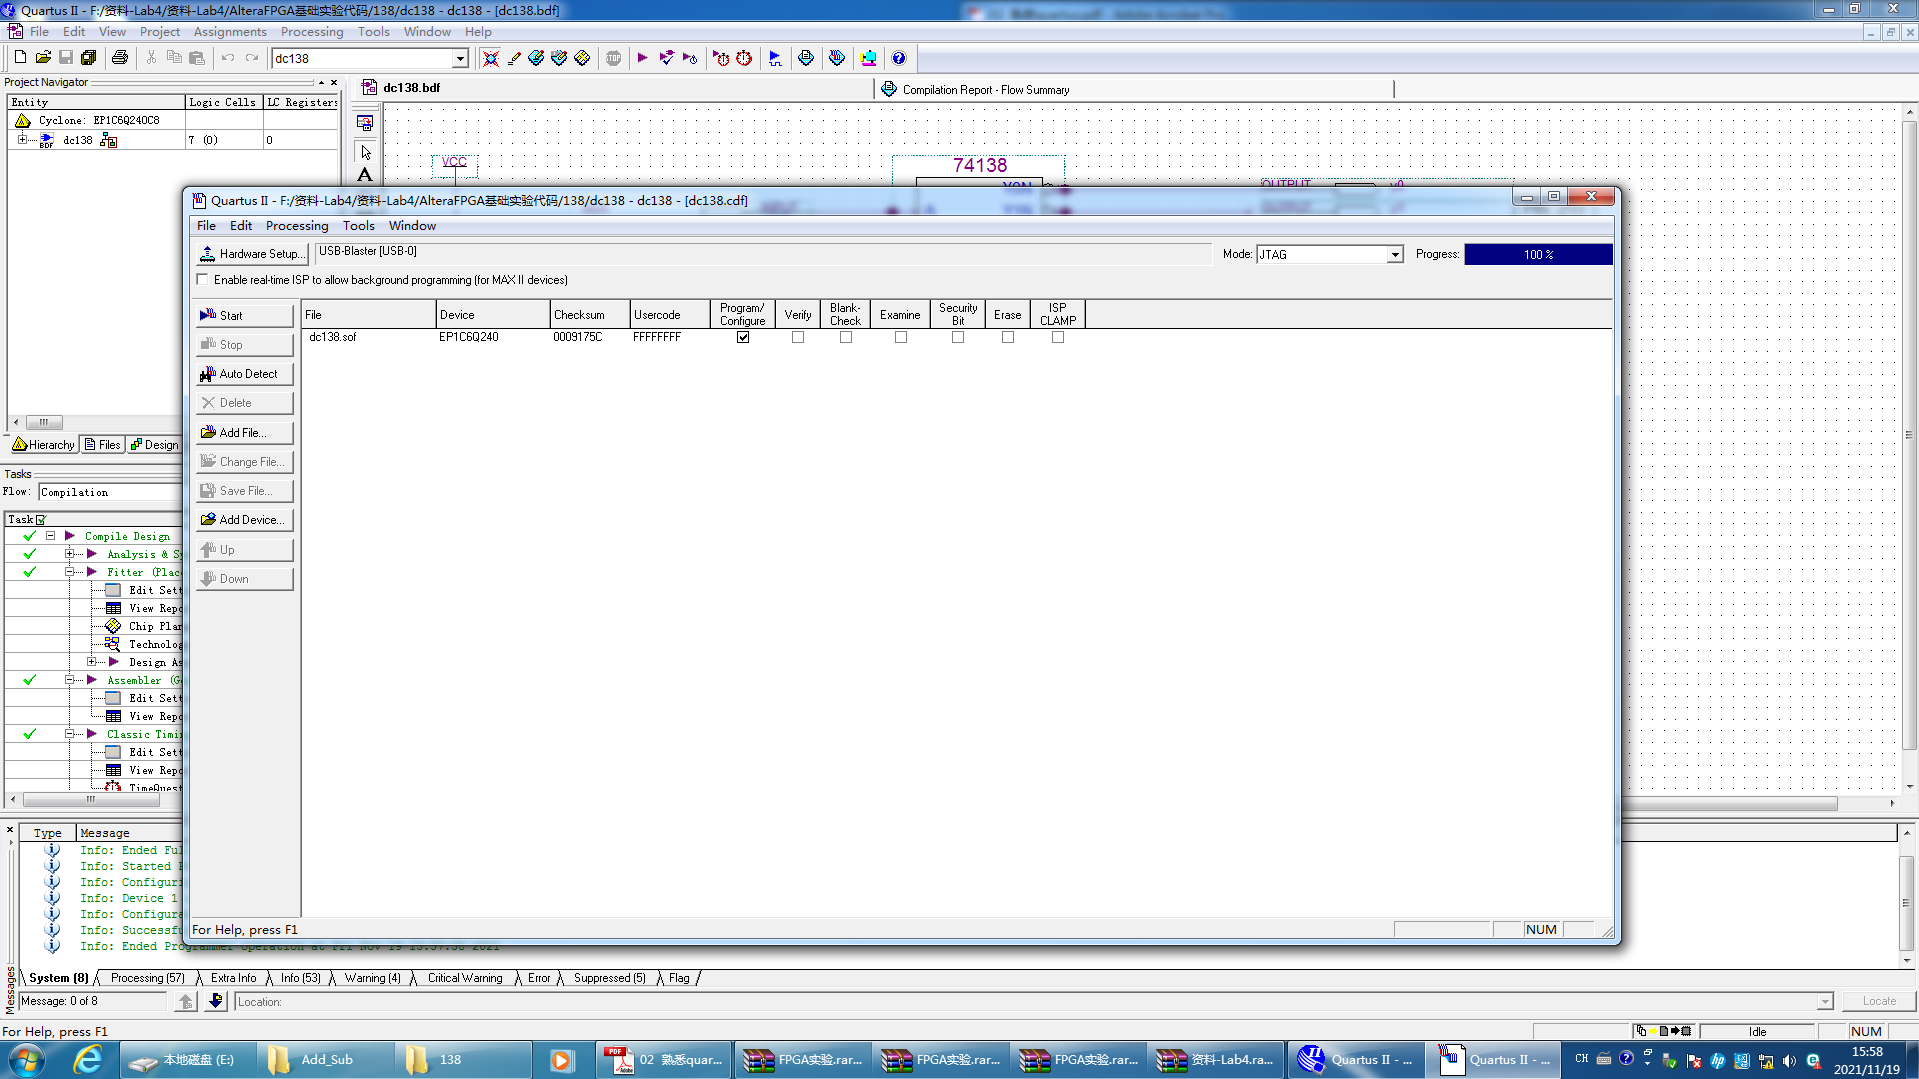
\includegraphics[width=\linewidth]{fig/Altera/9.PNG}
        \caption{烧录程序}
        \label{fig:Altera_9}
      \end{figure}

      \begin{figure}[htbp]
        \centering
        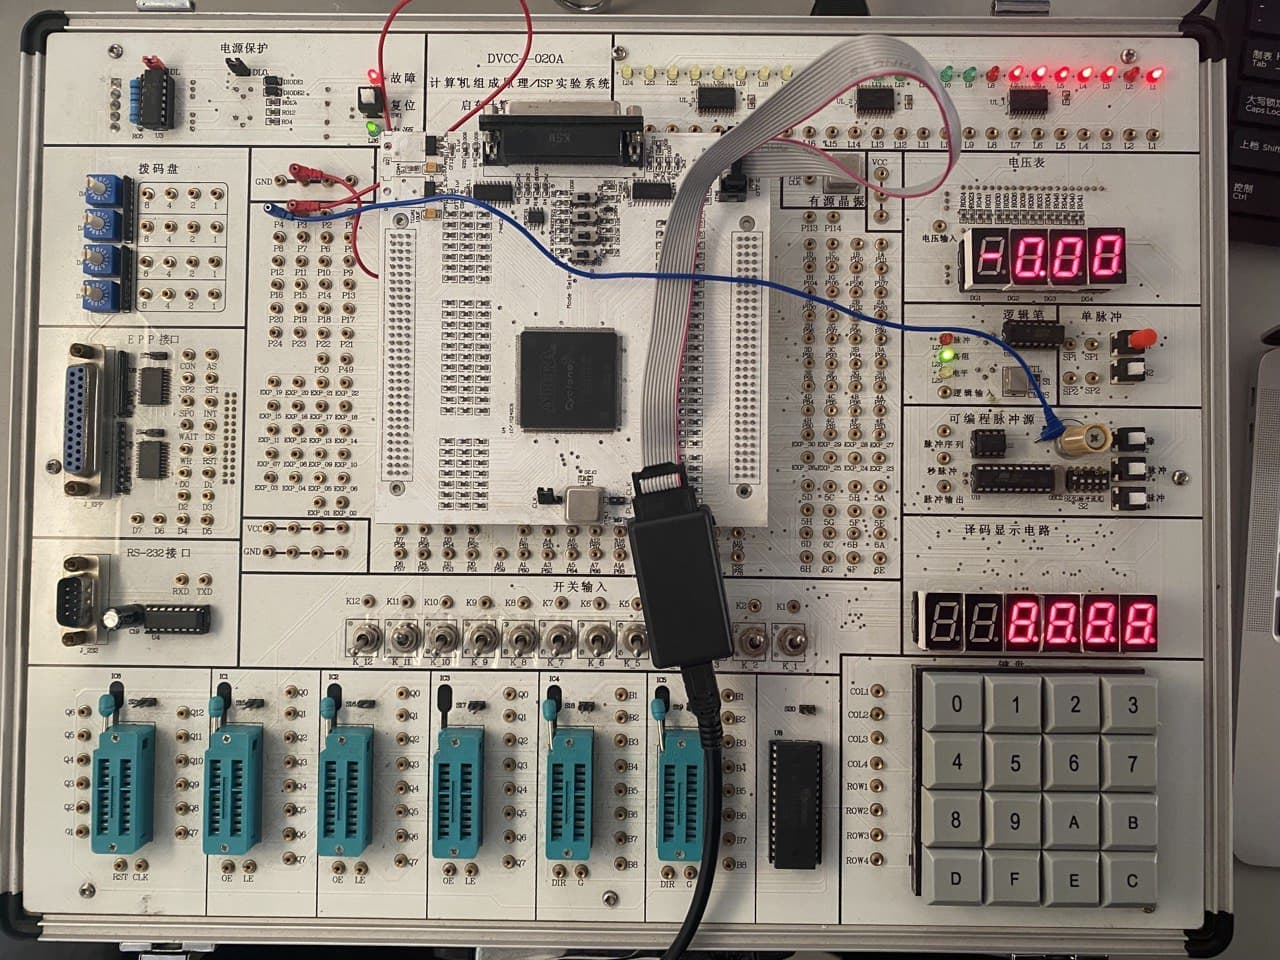
\includegraphics[width=.8\linewidth]{fig/Altera/result.jpg}
        \caption{Altera 实现结果}
        \label{fig:Altera_result}
      \end{figure}
    
    \newpage
    \section{选作探索与应用设计}

      Vivado 实现 上述 Altera 设计,由于手边没有合适的开发板,我只能在理论上分析这个结果.

      每一次 run 完 Implementation 后选择 Generate Bitstream 后可以选择烧录至开发板中,
      后面的过程应该是较为类似的,只是 Altera 的实现更多通过可视性的操作(和电路仿真软件 Multisim 较为接近),Vivado 可以将实现交给电脑来做.
      个人认为你 Vivado 在大工程项目的逻辑上更好掌握,即可以有一个明确的结构和互相调用的关系.

    \section{实验总结}

      这次实验内容较多,包括了 Vivado 和 Altera,其中 Vivado 基本都是课后完成的,实验室内完成了 Altera 实验.
      具体分析在各个部分都有,总体的感受是有些复杂的操作,我大为震撼,不过由于现在学习科研压力较大,没有能够更加深入其中做更多拓展的工作.
      不过目前对整个流程有一个大致的了解还是很好的锻炼,也为以后偏硬件的科研工作做好了铺垫.

      \begin{device}{}{devices}
        \begin{itemize}
          \item 清华科教仪器厂TPC-ZK-II\_PCI 微机接口实
          验装置
          \item EEEC-020A 计算机组成实验箱一台(自带电压表)
          \item RIGAL DG1022U 25MHz 双路波形发生器
          \item RIGOL DS1072E-EDU 70MHz 双踪数字记忆示波器
          \item Xilinx Vivado \textit{HLx} 2017.4
          \item Altera Quartus II 9.0
          \item Ubuntu 20 / Windows 11 / Windows 7{\kaishu\color{gray}(Vivado 实验于 Ubuntu 平台完成,Altera 实验于 Windows 7 上完成)}
        \end{itemize}
      \end{device}

    % 打印参考文献
    \addcontentsline{toc}{section}{参考文献}
    \printbibliography[sorting=none]

    % \newpage
    \addcontentsline{toc}{section}{附录 A:实验报告 \LaTeX 模板}
    \section*{附录 A:实验报告 \LaTeX 模板}

        实验报告使用自己编写的 \LaTeX 模板(\texttt{SEU-Digital-Report.cls}),
        在基本适配 Microsoft Word 版报告的格式要求之外,
        增加了更多的功能,使得报告看起来更加优雅多彩.

        后续升级后,报告模板将于 \url{https://github.com/Teddy-van-Jerry/TVJ-Digital-Report} 基于 MIT License 开源共享.

        编译需要使用 \texttt{XeLaTeX + Biber},封面页修改如下内容即可.
        \begin{lstlisting}[
          language=tex,
          morekeywords={
            expno,
            expname,
            expauthor,
            expID,
            expmates,
            expmatesID,
            expmajor,
            explab,
            expdate,
            expreportdate,
            expgrade,
            exptutor,
            today
          }
        ]
%% 使用实验报告模板类(字体大小 11pt 约为五号字)
\documentclass[11pt]{SEU-Digital-Report}

%%%%%%%%%%%%%%%%%%%% 报告基本信息 %%%%%%%%%%%%%%%%%%%%
\expno{四} % 实验序号
\expname{黑箱电路元件判别及参数测定} % 实验名称
\expauthor{赵舞穹} % 姓名
\expID{61520522} % 学号
\expmates{郑瑞琪} % 同组
\expmatesID{61520523} % 学号(同组)
\expmajor{工科试验班} % 专业
\explab{计算机硬件技术} % 实验室
\expdate{2021年11月19日} % 实验日期
\expreportdate{\today} % 实验日期
\expgrade{} % 成绩评定
\exptutor{冯熳} % 评阅教师
%%%%%%%%%%%%%%%%%%%%%%%%%%%%%%%%%%%%%%%%%%%%%%%%%%%%
        \end{lstlisting}

    \addcontentsline{toc}{section}{附录 B:Vivado 程序真伪判别}
    \section*{附录 B:Vivado 程序真伪判别}

    \begin{enumerate}
        \item Vivado 程序我在 Ubuntu 20.4 LTS 平台完成,标题栏为经典的 GNOME 桌面风格,与 Windows 有很大区别.
        \item 标题栏现实程序所在文件夹为 \texttt{/home/tvj/Documents/Verilog/SEU\_Digital\_Experiment},这是我的 GitHub 私有项目.
        \item Design Run 中显示的时间也可以辅助判断. (如图~\ref{fig:IP_RTL_detailed})
    \end{enumerate}

    \addcontentsline{toc}{section}{附录 C:Altera 程序真伪判别}
    \section*{附录 C:Altera 程序真伪判别}

    \begin{enumerate}
      \item Altera 程序我在实验室电脑上完成,是 Windows 7 版本,并且据我观察在课上完成 Altera 工作的不超过三组.
      \item 截图右下角时间为11月19日,是我们实验的时间.
      \item 我们有自己尝试的分配引脚的步骤,这其实超过了实验本身的要求.
    \end{enumerate}

\end{document}
